\section{Anwendung der Statistischen Physik}\marginpar{VL 18}

\subsection{Ideale Quantengase}
\begin{itemize}
    \item Gas aus identischen (vielen) Teilchen
    \item ideal: keine Wechselwirkungen
    \item Quantengase: quantenmechanishce Berücksichtigung, dass identische Teilchen ununterscheidbar sind
\end{itemize}

\begin{definition}{Einteilchen-Hamiltonoperator}
\begin{equation}
    \hat{h}_i \qquad \text{für das $i$-te Teilchen}
\end{equation}
\end{definition}
identisch für alle Teilchen ($h_i \equiv h$)

\begin{definition}{Einteilchen-Schrödinger-Gleichung}
    \begin{equation}
        \hat{h} \ket{k} = \varepsilon_k \ket{k}
    \end{equation}
\end{definition}
Einteilchen-Eigenenergien: $\varepsilon_0$, $\varepsilon_1$,... \\
Einteilchen Eigenzustände: $\ket{0}$, $\ket{1}$,...

\begin{definition}{N-Teilchen-Hamiltonoperator}
    \begin{equation}
        \hat{H} = \sum_{i=1}^N \ \hat{h}_i \qquad \text{(ohne WW, identische Teilchen)}
    \end{equation}
\end{definition}

\begin{definition}{N-Teilchen-Schrödinger-Gleichung}
    \begin{equation}
        \hat{H} \ket{k_1,k_2,...,k_N} = (\varepsilon_{k_1} + \varepsilon_{k_2} + ... + \varepsilon_{k_N}) \ket{k_1,k_2,...,k_N}
    \end{equation}
\end{definition}
N-Teilchen-Eigenenergie: $(\varepsilon_{k_1} + \varepsilon_{k_2} + ... + \varepsilon_{k_N})$\\
N-Teilchen-Eigenzustand: $\ket{k_1,k_2,...,k_N} = \ket{k_1}\cdot \ket{k_2} \dots \ket{k_N}$ (Produktzustand: 1. Teilchen in Zustand $\ket{k_1}$ usw.)

\begin{center}
    $\Longrightarrow$ Diese Eigenzustände sind nicht die physikalischen Eigenzustände!
\end{center}

\subsubsection{Ununterscheidbarkeit quantenmechanischer Teilchen}
Vergleich Stoß zweier identischer Teichen quantenmechanisch und klassisch:
\begin{center}
    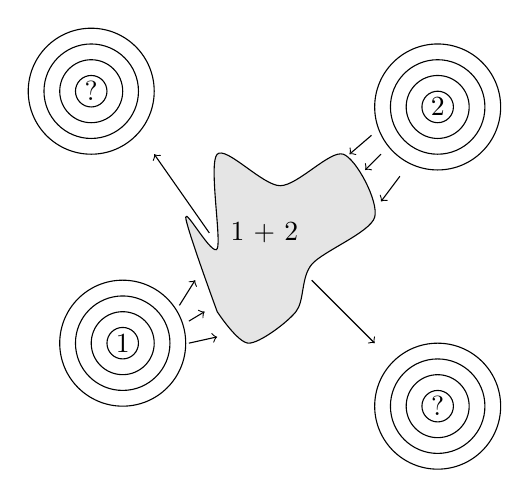
\begin{tikzpicture}[scale=0.4]
        \draw (0,0) circle (0.5);
        \draw (0,0) circle (1);
        \draw (0,0) circle (1.5);
        \draw (0,0) circle (2) node{1};
        \draw (10,7.5) circle (0.5);
        \draw (10,7.5) circle (1);
        \draw (10,7.5) circle (1.5);
        \draw (10,7.5) circle (2) node{2};
        \draw[fill=black!10] plot [smooth] coordinates{(3,1) (2,4) (3,3) (3,6) (5,5) (7,6) (8,4) (6,2.5) (5.5,1) (4,0) (3,1)};
        \draw (4.5,3.5) node{1 + 2};
        \draw[->] (1.8,1.2) -- (2.3,2);
        \draw[->] (2.1,0.7) -- (2.6,1);
        \draw[->] (2.1,0) -- (3,0.2);
        \draw[->] (8.2,6) -- (7.7,5.5);
        \draw[->] (7.9,6.6) -- (7.2,6);
        \draw[->] (8.8,5.3) -- (8.2,4.5);
        \draw[->] (6,2) -- (8,0);
        \draw[->] (2.75,3.5) -- (1,6);
        \draw (-1,8) circle (0.5);
        \draw (-1,8) circle (1);
        \draw (-1,8) circle (1.5);
        \draw (-1,8) circle (2) node{?};
        \draw (10,-2) circle (0.5);
        \draw (10,-2) circle (1);
        \draw (10,-2) circle (1.5);
        \draw (10,-2) circle (2) node{?};
    \end{tikzpicture}
    \hspace{3cm}
    \begin{tikzpicture}[scale=0.7]
        \draw plot [smooth] coordinates{(0,0) (2.5,2) (5,5)};
        \draw plot [smooth] coordinates{(2,-1) (4.5,2) (7,4)};
        \filldraw (0,0) circle (4pt) node[anchor=east]{1};
        \filldraw (7,4) circle (4pt) node[anchor=west]{2};
        \draw[<-] (5,5) -- (5.1,5,1);
        \draw[->] (2,-1) -- (1.9,-1.1);
    \end{tikzpicture}
\end{center}
\begin{multicols}{2}
    \textbf{qm:} Wellenpakete nach Stoß nicht merh den ursprünglichen Teilchen zuordenbar\\
    $\Rightarrow$ es ist sinnlos identische Teilchen zu nummerieren\\
    \textbf{klassisch:} man kann die Teilchen nummerieren und während des Stoßvorganges individuell verfolgen
\end{multicols}
\begin{center}
    $\Rightarrow$ weitreichende Konsequenzen
\end{center}

\subsubsection{Symmetrisierung}
\paragraph{Zwei-Teilchen-Zustände}
Teilchen-Vertauschungsoperator: $\widehat{P}_{12}$ (Austausch von Teilchen 1 und 2)

\begin{definition}{Teilchen-Vertauschungsoperator}
        \begin{align}
            \widehat{P}_{12} \ket{k_1,k_2} = \ket{k_2,k_1}
        \end{align}
\end{definition}
\begin{prop}{Eigenschaften des Teilchen-Vertauschungsoperators}
    \begin{align}
         &\rightarrow \widehat{P}_{12}\cdot \widehat{P}_{12} = \mathbb{1} \quad \Leftrightarrow \quad \widehat{P}_{12}^{-1} = \widehat{P}_{12}\\
            &\rightarrow \widehat{P}_{12} \text{ hermitesch, d.h. } \widehat{P}_{12}^{\dagger} = \widehat{P}_{12} \\
            &\rightarrow \text{Eigenwerte $\pi$ von }  \widehat{P}_{12} \ket{\varphi} = \pi \ket{\varphi} \ \text{ mit } \ (\widehat{P}_{12})^2 = \mathbb{1}\\
            &\qquad \Rightarrow \ket{\varphi} = \pi^2 \ket{\varphi} \ \Rightarrow \ \pi = \pm 1
    \end{align}
\end{prop}
\begin{proof}
    zur Hermitizität von $\widehat{P}_{12}$: Nutze Matrix in VON-Basis:
    \begin{align}
        \bra{k´,l´} \widehat{P}_{12} \ket{k,l} &= \bra{k´,l´}\ket{l,k} = \delta_{k´l}\delta_{l´k}  \label{eq:proof_hel_1}\\
        \bra{k´,l´} \widehat{P}_{12}^{\dagger} \ket{k,l} &= (\bra{k,l}\widehat{P}_{12}\ket{k´,l´})^* \\
        &= (\bra{k,l}\ket{l´,k}´)^* =\bra{l´,k´}\ket{k,l} = \delta_{l´k}\delta_{k´l} \label{eq:proof_hel_2}\\
        &\Longrightarrow (\ref{eq:proof_hel_1}) = (\ref{eq:proof_hel_2})
    \end{align}
\end{proof}

Sei $A$ eine Observable, die nicht zwischen Teilchenunterscheidet:
\begin{align}
    A \ket{k_1,k_2} &\stackrel{!}{=} \widehat{P}_{12}^{-1} \, A \, \widehat{P}_{12} \ket{k_1,k_2} \\
    &\Rightarrow A = \widehat{P}_{12}^{-1} \, A \, \widehat{P}_{12} \ \Rightarrow \ \widehat{P}_{12} A = A \widehat{P}_{12} \ \Rightarrow \ [A,\widehat{P}_{12}]=0
\end{align}
$H=\sum_i h_i$ macht keine Unterscheidung zwischen Teilchen (da $h \equiv h_i$)
\begin{itemize}
    \item[$\Rightarrow$] $[H,\widehat{P}_{12}]=0$
    \item[$\Rightarrow$] $\exists$ vollständiger Satz gemeinsamer Eigenzustände 
    \item[$\Rightarrow$] diese Eigenzustände sind in 2 Klassen einteilbar:
    \begin{align}
        \pi = +1 : \quad \ket{k_1,k_2}&+\ket{k_2,k_1} \quad \text{symmetrisch unter Vertauschung}\\
        \color{black!40} \widehat{P}_{12}\ket{k_1,k_2}&\color{black!40}+\widehat{P}_{12}\ket{k_2,k_1} = (+1)\cdot\ket{k_1,k_2} + (+1) \cdot \ket{k_2,k_1}\\
        \pi = -1 : \quad \ket{k_1,k_2}&-\ket{k_2,k_1} \quad \text{antisymmetrisch unter Vertauschung}\\
        \color{black!40} \widehat{P}_{12}\ket{k_1,k_2}&\color{black!40}-\widehat{P}_{12}\ket{k_2,k_1} = (-1)\cdot\ket{k_1,k_2} \underbrace{- (-1)}_{=+1} \cdot \ket{k_2,k_1}\\
        &\rightarrow \text{diese Zustände gibt es nur für } k_1 \neq k_2\\
        &\color{green!70!black} \rightarrow \text{Pauli-Prinzip} \color{black}
    \end{align}
\end{itemize}
Das Experiment zeigt, dass jeweils nur eine Klasse von Eigenzuständen auftritt!
\begin{beispiel}{Analogie zum unendlichen Kastenpotential}
\begin{multicols}{2}
    \begin{center}
    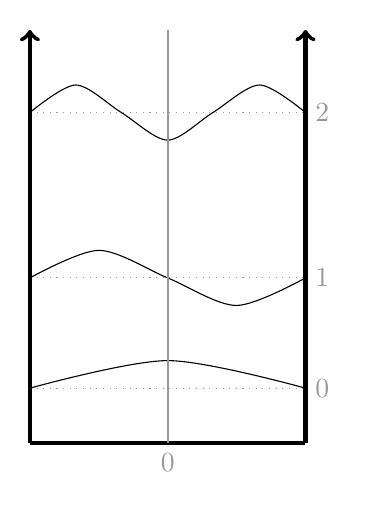
\begin{tikzpicture}[scale = 0.7]
        \draw[ultra thick,->] (0,0) -- (0,7.5);
        \draw[ultra thick,->] (5,0) -- (5,7.5);
        \draw[ultra thick] (0,0) -- (5,0);
        \draw[dotted,black!40] (0,1) -- (5,1) node[anchor=west]{0};
        \draw plot [smooth] coordinates{(0,1) (2.5,1.5) (5,1)};
        \draw[dotted,black!40] (0,3) -- (5,3) node[anchor=west]{1};
        \draw plot [smooth] coordinates{(0,3) (1.25,3.5) (2.5,3) (3.75,2.5) (5,3)};
        \draw[dotted,black!40] (0,6) -- (5,6) node[anchor=west]{2};
        \draw plot [smooth] coordinates{(0,6) (0.83,6.5) (1.66,6) (2.5,5.5) (3.32,6) (4.17,6.5) (5,6)};
        \draw[thick, black!40] (2.5,7.5) -- (2.5,0) node[anchor=north]{0};
    \end{tikzpicture}
    \end{center}
    \begin{itemize}
        \item[] Spiegelung um null
        \item[] 1.Klasse: nur symmetrisch
        \begin{itemize}
            \item[$\rightarrow$] Eigenzustände 0,2,4,...
        \end{itemize}
        \item[] 2. Klasse: nur antisymmetrisch
        \begin{itemize}
            \item[$\rightarrow$] Eigenzustände 1,3,5,...
        \end{itemize}
    \end{itemize}
\end{multicols}
\end{beispiel}

\begin{definition}{Symmetrisierungspostulat}
    Alle Zustände eines Systems aus identischen Teilchen sind unter Vertauschung entweder vollkommen symmetrisch und man nennt die Teilchen \emph{Bosonen} oder vollkommen antisymmetrisch und man nennt sie \emph{Fermionen}.
\end{definition}

\paragraph{Empirische Regel (Spin-Statistik-Theorem)}
\begin{itemize}
    \item Teilchen mit halbzahligem Spin ($\frac{1}{2},\frac{3}{2},..$) sind Fermionen
    \begin{itemize}
        \item Leptonen ($e,\mu,\tau,\nu_e,\nu_{\mu},\nu_{\tau}$) und Quarks ($u,d,s,c,b,t$)
    \end{itemize}
    \item Teilchen mit ganzzahligem Spin (0,1,2,...) sind Bosonen
    \begin{itemize}
        \item WW vermittelnden Teilchen:
        \begin{itemize}
            \item[] elm. WW: Photonen $\gamma$
            \item[] schwache WW: $W^{\pm}$, $Z^0$
            \item[] starke WW: Gluonen $g$
            \item[] Gravitation: Graviton 
        \end{itemize}
        \item kollektive Anregungen: Phononen, Plasmonen, Magnonen,...
        \item zusammengesetzte Teilchen:
        \begin{itemize}
            \item ungerade Anzahl Fermionen + beliebig viele Bosonen $\Rightarrow$ Fermion
            \begin{itemize}
                \item[] Baryonen (3 Quarks): Neutron, Proton
                \item[] $^3He$ (2 Protonen, 1 Neutron, 2 Elektronen) 
            \end{itemize}
            \item gerade Anzahl Fermionen + beliebig viele Bosonen $\Rightarrow$ Boson
            \begin{itemize}
                \item[] Mesonen (2 Quarks): Charmonium
                \item[] $^4He$ (2 Protonen, 2 Neutronen, 2 Elektronen) 
            \end{itemize}
        \end{itemize}
    \end{itemize}
\end{itemize}

\paragraph{Drei-Teilchen-Zustände}
\begin{itemize}
    \item[] Bosonen ($\pi=+1$, vollkommene Symmetrie)
    \begin{itemize}
        \item[*] $k_1 \neq k_2$, $k_1 \neq k_3$, $k_2 \neq k_3$
        \begin{equation}
            \ket{k_1,k_2,k_3} + \ket{k_2,k_3,k_1} + \ket{k_3,k_1,k_2} + \ket{k_2,k_1,k_3} + \ket{k_3,k_2,k_1} + \ket{k_1,k_3,k_2}
        \end{equation}
        \item[*] $k_1 = k_2 = k$, $k_3 \neq k$
        \begin{equation}
            \ket{k,k,k_3} + \ket{k_3,k,k} + \ket{k,k_3,k}
        \end{equation}
        \item[*] $k_1=k_2=k_3=k$
        \begin{equation}
            \ket{k,k,k}
        \end{equation}
    \end{itemize}
    \item[] Fermionen ($\pi = -1$, vollkommen antisymmetrisch)
    \begin{itemize}
        \item[*] $k_1 \neq k_2$, $k_1 \neq k_3$, $k_2 \neq k_3$
        \begin{align}
            \ket{k_1,k_2,k_3} + &\ket{k_2,k_3,k_1} + \ket{k_3,k_1,k_2} - \ket{k_2,k_1,k_3} - \ket{k_3,k_2,k_1} - \ket{k_1,k_3,k_2}\\
            &= det\begin{pmatrix}
                \ket{k_1} & \ket{k_1} & \ket{k_1}\\
                \ket{k_2} & \ket{k_2} & \ket{k_2}\\
                \ket{k_3} & \ket{k_3} & \ket{k_3}
            \end{pmatrix}
        \end{align}
        \item[*] keine weiteren Zustände
    \end{itemize}
\end{itemize}
\subparagraph{Bemerkung}
Es gibt mehr Mikrozustände für Bosonen als für Fermionen!

\paragraph{Vielteilchenzustände}
\begin{itemize}
    \item Bosonen ($\pi = +1$, vollkommen symmetrisch):\\
    alle $k_i$ unterschiedlich ($k_n\neq k_m$ $\forall n\neq m$)
    \begin{align}
        \frac{1}{\sqrt{N!}} \sum_{\gamma =1}^{N!} P_{\gamma} \ket{k_1,k_2,...,k_N} \quad P_{\gamma}\text{ erzeuge alle N' Permutationen}
    \end{align}
    einige der $k_i$ haben gleiche Werte $k_j$ kommt $n_j$ mal vor, $j=1,...,J<N$
    \begin{align}
        \frac{1}{\sqrt{S}} \sum_{\gamma = 1}^S P'_{\gamma} \ket{k_1,k_2,...,k_N} \quad P'_{\gamma} \text{ erzeuge alle Permutationen der Dopplung}\\
        S=\frac{N!}{n_1!n_2!...n_J!}
    \end{align}
    \item Fermionen ($\pi = -1$, vollkommen antisymmetrisch):
    \begin{align}
        \frac{1}{\sqrt{N!}} \sum_{\gamma =1}^{N!} (-1)^{\tau} P_{\gamma} \ket{k_1,k_2,...,k_N} 
        =\frac{1}{\sqrt{N}} \underbrace{\det \mqty(\ket{k_1} & \ket{k_1} & ... & \ket{k_1} \\ \ket{k_2} & \ket{k_2} & ... & \ket{k_2} \\ ... & ... & &... \\ \ket{k_N} & \ket{k_N} & ... & \ket{k_N})}_{\text{Slater-Determinante}}
    \end{align}
    hier darf kein $k_i=k_j$ sein, sonst zwei gleiche Zeilen in Determinante $\Rightarrow$ Zustand verschwindet: Pauli-Prinzip
\end{itemize}
\subparagraph{Anmerkung}
Diese Schreibweise der Symmetrisierung wird hier nicht gebraucht



\subsubsection{Fockraum, Besetzungszahldarstellung} \marginpar{VL 19}

\paragraph{Ziel:} Schreibweise ohne umständliche Symmtrisierung
\begin{definition}{Fockraum}
    Betrachte Einteilchenzustände $\ket{0},\ket{1},...$ und gebe an, mit wie vielen Teilchen besetzt\\
    $\Rightarrow$ Besetzungszahl $n_k$ des Einteilchenzustands $\ket{k}$\\
    $\Rightarrow$ $\ket{n_0,n_1,n_2,...,n_k,...}$ ist Zustand in Fockraum ($\ket{n_0}=$ Teilchen im Einteilchenzustand $\ket{0}$)
\end{definition}


\begin{beispiel}{Beispiele}
    \begin{itemize}
        \item $\ket{n_0,n_1,n_2,...,n_k,...}$ ist Zustand im Fockraum
        \begin{itemize}
            \item[] mit $n_0$ im Einteilchen-Grundstustand $\ket{0}$,
            \item[] ...,
            \item[] mit $n_k$ im Einteilchen-Zustand $\ket{k}$,
            \item[] ...
        \end{itemize}
        \item Vakuum: $\ket{0,0,0,...}$
        \item Einteilchenzustand $\ket{k}$: $\ket{0,0,...,0,1,0,...}$
    \end{itemize}
\end{beispiel}
\paragraph{Bemerkung:}
\begin{itemize}
    \item Zahl der Teilchen nicht festgelegt
    \item Bosonen: $n_k = 0,1,2,...$
    \item Fermionen: $n_k = 0,1$
    \item Symmetrisierung (damit) berücksichtigt
\end{itemize}



\begin{definition}{Besetzungszahloperator $\hat{n}_k$}
    \begin{align}
        \hat{n}_k \ket{n_0,n_1,...,n_k}= n_k \ket{n_0,n_1,...,n_k,...}
    \end{align}
\end{definition}
\color{black!40}
Später:
    \begin{align}
        \hat{n}_k = a_k^+a_k
    \end{align}
    Man nennt dies auch die 2. Quantisierung (erst Einteilchezustände $\ket{k}$ und jetzt $n_k$ als Quantenzahlen). Die $a_k$ sind dabei für Fermionen und Bosonen unterschiedlich (siehe Quantentheorie 2).
\color{black}

\begin{definition}{Teilchenzahloperator}
    \begin{align}
        \hat{N} = \sum_{k=0}^{\infty} \hat{n}_k
    \end{align}
\end{definition}

\begin{definition}{Hamiltionoperator mit Besetzungszahloperator}
    \begin{align}
        \hat{H} = \sum_k \hat{n}_k \varepsilon_k
    \end{align}
\end{definition}


\begin{beispiel}{2 Niveau System}
    Einteilchenzustände $\ket{a},\ket{b}$
    \begin{multicols}{2}
       \begin{itemize}
        \item 1 Teilchen ($\ket{a},\ket{b}$:\\
        Einteilchen-Darst.: $\ket{a},\ket{b}$\\
        Besezungszahl.: $\ket{1,0},\ket{0,1}$
        \item Teilchen, Bosonen\\
        Zweiteilchen-Darst.: $\ket{a,a} \frac{1}{\sqrt{2}}(\ket{a,b}-\ket{b,a}) \ket{b,b}$\\
        Besetzungsgrad.: $\ket{2,0} \ket{1,1} \ket{0,2}$\\
        $\Rightarrow$ 3 Zustände
        \item 2 Teilchen, Fermionen\\
        Zweiteilchen-Darst.: $\frac{1}{\sqrt{2}}(\ket{a,b}-\ket{b,a})$\\
        Besetzungszahl.: $\ket{1,1}\\
        \Rightarrow$ 1 Zustand
        \item 2 Teilchen, klassische unterscheidbar\\
        Klass. Berücksichtigung der Ununterscheidbarkeit: Faktor $\frac{1}{N!}$\\
        $\Rightarrow$ 2 Zustände
        $\Rightarrow$ M-B-Stat.
        \end{itemize} 
        \begin{center}
            \begin{tikzpicture}[scale = 0.5]
                \draw[thick,red] (3,0) -- (0,0) node[anchor=east]{$\varepsilon_a$};
                \draw[thick,red] (3,1) -- (0,1) node[anchor=east]{$\varepsilon_b$};
                \filldraw[black] (1,0) circle (3pt);
                \filldraw[green] (2,0) circle (3pt);
                \draw[thick,red] (4,0) -- (7,0);
                \draw[thick,red] (4,1) -- (7,1);
                \filldraw[black] (5,0) circle (3pt);
                \filldraw[green] (6,1) circle (3pt);
                \draw[thick,red] (8,0) -- (11,0);
                \draw[thick,red] (8,1) -- (11,1);
                \filldraw[black] (9,1) circle (3pt);
                \filldraw[green] (10,0) circle (3pt);
                \draw[thick,red] (12,0) -- (15,0);
                \draw[thick,red] (12,1) -- (15,1);
                \filldraw[black] (13,1) circle (3pt);
                \filldraw[green] (14,1) circle (3pt);
                
                \draw[thick,red] (3,4) -- (0,4) node[anchor=east]{$\varepsilon_a$};
                \draw[thick,red] (3,5) -- (0,5) node[anchor=east]{$\varepsilon_b$};
                \filldraw[black] (1.5,4) circle (3pt);
                \filldraw[black] (1.5,5) circle (3pt);
                
                \draw[thick,red] (3,8) -- (0,8) node[anchor=east]{$\varepsilon_a$};
                \draw[thick,red] (3,9) -- (0,9) node[anchor=east]{$\varepsilon_b$};
                \filldraw[black] (1,8) circle (3pt);
                \filldraw[black] (2,8) circle (3pt);
                \draw[thick,red] (4,8) -- (7,8);
                \draw[thick,red] (4,9) -- (7,9);
                \filldraw[black] (5,8) circle (3pt);
                \filldraw[black] (6,9) circle (3pt);
                \draw[thick,red] (8,8) -- (11,8);
                \draw[thick,red] (8,9) -- (11,9);
                \filldraw[black] (9,9) circle (3pt);
                \filldraw[black] (10,9) circle (3pt);

                \draw[thick,red] (3,12) -- (0,12) node[anchor=east]{$\varepsilon_a$};
                \draw[thick,red] (3,13) -- (0,13) node[anchor=east]{$\varepsilon_b$};
                \filldraw[black] (1.5,12) circle (3pt);
                \draw[thick,red] (4,12) -- (7,12);
                \draw[thick,red] (4,13) -- (7,13);
                \filldraw[black] (5.5,13) circle (3pt);
            \end{tikzpicture}
        \end{center}
    \end{multicols}
     
\end{beispiel}
\begin{itemize}
    \item[$\rightarrow$] Besetzungszahldarstellung für klassische Teilchen nicht möglich
    \item[$\rightarrow$] klassische Berücksichtigung der Ununterscheidbarkeit durch Faktor $\frac{1}{N!}$ (Maxwell-Boltzmann-Statistik $\Rightarrow$ effektiv 2 Zustände (liegt zwischen Fermionen und Bosonen))
\end{itemize}


\subsubsection{Zustandssumme}
kanonische Zustandssumme für $N$ Teilchen: $Z=\trace\left(e^{-\beta H}\right)$
\begin{align}
    Z =\trace\left(e^{-\beta H}\right)&= \sum_{n_0,n_1,...}\ev{e^{-\beta \sum_k \varepsilon_k \hat{n}_k}}{n_0,n_1,...} \quad \text{mit} \sum_k n_k=N\\
    &= \sum_{n_0,n_1,...} e^{-\beta \sum_k \varepsilon_k n_k} = \sum_{n_0,n_1,...} \prod_k e^{-\beta \varepsilon_k n_k}\\
    &\rightarrow \text{weitere Umformungen wegen Summeneinschränkung schwierig}
\end{align}

\begin{beispiel}{2 Einteilchenzustände}
    N=3 $\Rightarrow$ $\ket{3,0}, \ \ket{2,1}, \ \ket{1,2},\ \ket{0,3}$
\end{beispiel}

großkanonische Zustandssumme:
\begin{itemize}
    \item Vorteil: N beliebig $\Rightarrow$ keine Einschränkung an Summe
    \item Nachteil: chem. Potential $\mu$ statt N
\end{itemize}
\begin{align}
    Z_G =  \trace\left( e^{-\beta (\hat{H}-\mu) \hat{N}}\right)&= \underbrace{\sum_{n_0,n_1,...}}_{\text{bel. Besetz. ET-Zustände}} \ev{e^{-\beta ( \sum_k (\varepsilon_k-\mu) \hat{n}_k)}}{n_0,n_1,...}\\
    &= \sum_{n_0,n_1,...} e^{-\beta \sum_k(\varepsilon_k-\mu)n_k}=\sum_{n_0,n_1,...} \prod_k \underbrace{e^{-\beta(\varepsilon_k-\mu)n_k}}_{(X_n)^{n_k}} \\
    &\overset{*}{=} \prod_k \sum_{n_k} (X_n)^{n_k}
\end{align}
zu ($*$)
\begin{align}
    (X_0)^0\cdot(X_1)^0 &+ (X_0)^1\cdot(X_1)^0 + (X_0)^0\cdot(X_1)^1 + (X_0)^2\cdot(X_1)^0 + (X_0)^1\cdot(X_1)^1 + (X_0)^0\cdot(X_1)^2 + ... \\
    &= \left[ (X_0)^0 + (X_0)^1 + (X_0)^2 + ... \right] \left[ (X_1)^0 + (X_1)^1 + (X_1)^2 + ... \right]
\end{align}
$\rightarrow$ Vertauschung von $\Sigma$ und $\Pi$ nur möglich, da N beliebig\\
(richtig: Reihe konvergent, da Zustände und e-Fkt. > 0 $\Rightarrow$ absolut konvergent $\Rightarrow$ Cauchy-Produkt)\\
\textbf{Fermionen:}
\begin{align}
    \sum_{n_k=0,1} (X_k)^{n_k} = 1 + X_k
\end{align}
\begin{definition}{Zustandssumme Fermionen}
    \begin{align}
        Z_G = \prod_k (1+ e^{-\beta(\varepsilon_k - \mu)})
    \end{align}
\end{definition}
\textbf{Bosonen:}
\begin{align}
    \sum_{n_k=0}^\infty (X_k)^{n_k} = \frac{1}{1-X_k}
\end{align}
\begin{definition}{Zustandssumme Bosonen}
    \begin{align}
        Z_G = \prod_k \frac{1}{1-e^{-\beta(\varepsilon_k-\mu)}}
    \end{align}
    gilt nur falls: $ \abs{X_k}<1 \Leftrightarrow \beta(\varepsilon_k-\mu) > 0 \Leftrightarrow \mu < \varepsilon_k \forall k$ insbesondere $\mu < \varepsilon_0$ Grundzustandsenergie. Dies ist eine phy. sinnvolle Einschränkung, da sonst $\infty$ Bosonen im Grundzustand (kein GG möglich, da alle Teilchen aus Reservoir in Grundzustand gehen würden)
\end{definition}

\subsubsection{Großkanonisches Potential und mittlere Besetzungszahl} \marginpar{VL 20}

\begin{definition}{Großkanonisches Potential}
    \begin{equation}
        \Phi(\beta,V,\mu) = - \frac{1}{\beta} \ln(Z_G) = \mp \frac{1}{\beta} \sum_k \ln\left(1 \pm e^{-\beta(\varepsilon_k-\mu)}\right)
    \end{equation}
\end{definition}
\begin{center}
    (oberes VZ Fermionen, unteres VZ Bosonen ($\mu < \varepsilon_0$))
\end{center}
Bemerkung: $\beta$, $\mu$ explizit, V beeinflusst Einteilchenenergien $\varepsilon_k$
\begin{center}
    $\Longrightarrow$ alle thermodynamischen Eigenschaften berechenbar
\end{center}
\begin{align}
    \Phi(T,V,\mu) &= U - TS -\mu N\\
    d\Phi &= - S \ dT - p \ dV - N \ d\mu
\end{align}

\paragraph{mittlere Teilchenzahl}
\begin{equation}
    \expval{\hat{N}}(\beta,V,\mu) = - \left(\pdv{\Phi}{\mu}\right)_{T,V} = \pm \frac{1}{\beta} \sum_k \frac{\pm e^{-\beta(\varepsilon_k-\mu)}\cdot \beta}{1 \pm e^{-\beta(\varepsilon_k-\mu)}} = \sum_k \frac{1}{e^{\beta(\varepsilon_k-\mu)}\pm 1}
\end{equation}
$\rightarrow$ Zusammenhang mittlere Teilchenzahl und chemisches Potential

\paragraph{mittlere Besetzungszahl von Einteilchenzustand $k$}
\begin{align}
    \qq*{vergleiche:} \expval{\hat{N}} &= \sum_k \expval{\hat{n}_k} \qq{(Annahme)} \\
    \Longrightarrow \quad \expval{\hat{n}_k} &=
    \begin{cases}
        \frac{1}{e^{\beta(\varepsilon_k-\mu)}+1} \qquad \text{Fermionen: Fermi-Dirac-Statistik} \\
        \frac{1}{e^{\beta(\varepsilon_k-\mu)}-1} \qquad \text{Bosonen: Bose-Einstein-Statistik } (\mu< \varepsilon_0)
    \end{cases}
\end{align}

Jetzt explizite Rechnung:
\begin{align}
    \expval{\hat{n}_k} = \trace(\hat{\varrho}\hat{n}_k) &= \sum_{n_0,n_1,...} n_k \, p(\ket{n_0,n_1,..})\\ \color{black!50}
    \hat{\varrho} &= \color{black!50}\frac{e^{-\beta(\hat{H}-\mu\hat{N})}}{Z_G} \\
    \color{black!50}p(\ket{n_0,n_1,...}) &= \color{black!50}\frac{1}{Z_G} e^{-\beta \sum_k (\varepsilon_k-\mu)n_k}\\
    &= \frac{1}{Z_G} \sum_{n_0,n_1,..} n_k \, e^{-\beta \sum_k (\varepsilon_k-\mu)n_k}\\
    &= \frac{1}{Z_G} \left(-\frac{1}{\beta} \right) \pdv{\varepsilon_k} \underbrace{\sum_{n_0,n_1,...} e^{-\beta \sum_k (\varepsilon_k-\mu)n_k}}_{Z_G} = -\frac{1}{\beta} \pdv{\varepsilon_k} \ln(Z_G)\\
    &= -\frac{1}{\beta} \pdv{\varepsilon_k} \ln\left(\left(1 \pm e^{-\beta(\varepsilon_k-\mu)}\right)^{\pm 1} \right) = - \frac{1}{\beta} \frac{e^{-\beta(\varepsilon_k-\mu)} \cdot (-\beta)}{1 \pm e^{-\beta(\varepsilon_k-\mu)}} \\
    &= \frac{1}{e^{+\beta(\varepsilon_k-\mu)}\pm 1} \qquad \checkmark
\end{align}
\begin{center}
    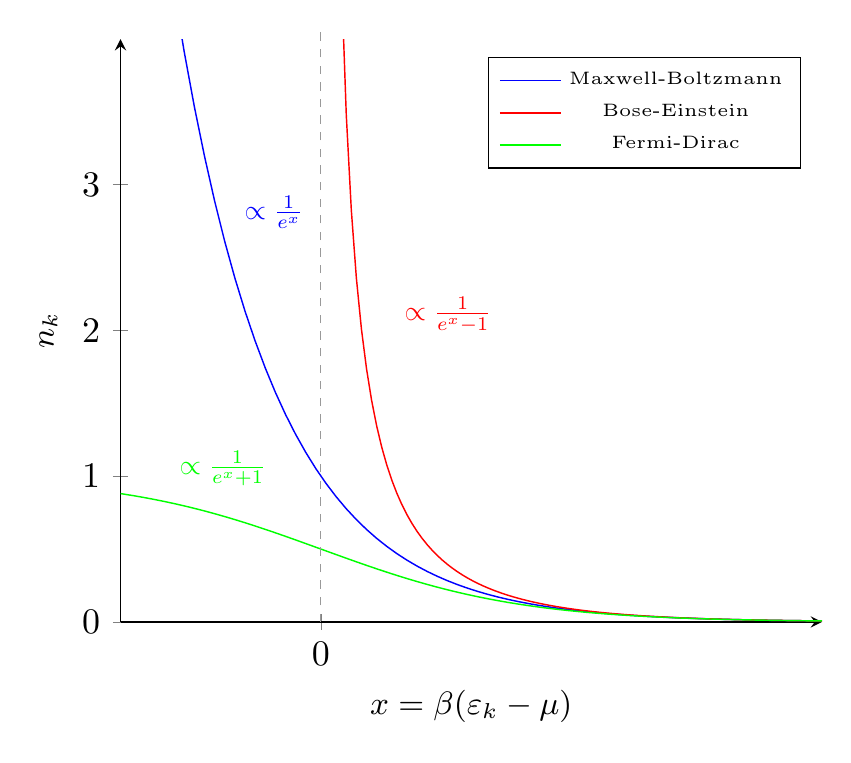
\begin{tikzpicture}[scale=1.3]
        \begin{axis}[
        axis lines = left,
        xlabel ={\small $x=\beta (\varepsilon_k-\mu)$},
        ylabel = {\small $\expval{n_k}$},
        xmin= -2, xmax=5,
        ymin=0, ymax=4,
        xtick = {0}, xticklabels = {0},
        ytick={0,1,2,3}, yticklabels= {0,1,2,3},
        legend pos=north east,
        ]
        \addplot[samples=100, color=blue]{1/(e^x)};
        \addplot[domain=0:5, samples=100, color=red]{1/(e^x-1)};
        \addplot[samples=100, color=green]{1/(e^x+1)};
        \legend{\tiny Maxwell-Boltzmann, \tiny Bose-Einstein, \tiny Fermi-Dirac}
        \end{axis}
        \draw[red] (3.2,3) node{$\propto \frac{1}{e^x-1}$};
        \draw[blue] (1.5,4) node{$\propto \frac{1}{e^x}$};
        \draw[green] (1,1.5) node{$\propto \frac{1}{e^x+1}$};
        \draw[dashed, black!40] (1.95,0) -- (1.95,5.8);
    \end{tikzpicture}
\end{center}
\begin{itemize}
    \item[] Besetzungszahl $n_k \ll 1$ (geringe Teilchendichte)
    \begin{itemize}
        \item[$\Rightarrow$] Statistik gleich 
    \end{itemize}
    \item[] Besetzungszahl $n_k \gg 1$ (Bosonen, hohe Teilchendichte) oder $n_k \approx 1$ (Fermionen)
    \begin{itemize}
        \item[$\Rightarrow$] neue Quantenphänomene für Fermionen / Bosonen 
    \end{itemize}
\end{itemize}

\begin{center}
    \begin{tikzpicture}
        \draw[ultra thick, <-] (0,7) -- (0,0) node[anchor=north]{Fermionen};
        \draw[ultra thick, <-] (7,7) -- (7,0) node[anchor=north]{Bosonen};
        \draw[ultra thick] (6.9,5.5) -- (7.1,5.5) node[anchor=west]{$\varepsilon_0$};
        \draw[ultra thick] (0.1,1) -- (-0.1,1) node[anchor=east]{$\varepsilon_0$};
        \draw[ultra thick] (0.1,2) -- (-0.1,2) node[anchor=east]{$\varepsilon_1$};
        \draw[ultra thick] (0.1,3) -- (-0.1,3) node[anchor=east]{$\varepsilon_2$};
        \draw[ultra thick] (0.1,4) -- (-0.1,4) node[anchor=east]{$\varepsilon_3$};
        \draw[ultra thick] (0.1,5) -- (-0.1,5) node[anchor=east]{$\varepsilon_4$};
        \draw[ultra thick] (0.1,6) -- (-0.1,6) node[anchor=east]{$\varepsilon_5$};
        \draw[thick, black!40] (1,4.5) -- (6,4.5) node[anchor=north west]{$\mu$};
        \fill[black!40, pattern=north east lines] (1,0) rectangle (6,4.5);
        \draw[thick] (0.5,4.5) -- (0.5,1);
        \draw[thick] (0.4,4.5) -- (0.6,4.5);
        \draw[thick] (0.4,1) -- (0.6,1);
        \draw[thick] (6.5,4.5) -- (6.5,5.5);
        \draw[thick] (6.4,4.5) -- (6.6,4.5);
        \draw[thick] (6.4,5.5) -- (6.6,5.5);
        \draw[black!60] (0,-1) node{(je ein Teilchen in Zuständen};
        \draw[black!60] (0,-1.5) node{mit $\varepsilon_k < \mu$)};
        \draw[black!60] (7,-1) node{(Divergenz $\widehat{=}$};
        \draw[black!60] (7,-1.5) node{immer mehr Teilchen würden};
        \draw[black!60] (7,-2) node{in Grundzustand gelangen)};
        
    \end{tikzpicture}
\end{center}

\subparagraph{Bemerkung:}
\begin{itemize}
    \item physikalische Bedeutung von $x \gg 1 \, \Leftrightarrow \ \varepsilon_0-\mu \gg kT$ (bei wenigen Teilchen ist Unterschied zwischen Fermionen und Bosonen gering)
    \begin{itemize}
        \item[$\rightarrow$] nicht zu interpretieren als $T \to 0$, sondern als $n_k \to 0$, d.h. klassischer Grenzfall 
    \end{itemize}
    \item weitere Größen:
    \begin{equation}
        p = \left(\pdv{\Phi}{V}\right)_{T,\mu} \qquad S = - \left( \pdv{\Phi}{T}\right)_{V,\mu}
    \end{equation}
    \item thermische Zustandsgleichung und Adiabatengleichung $\rightarrow$ Übung 12.2
\end{itemize}

\subsubsection{Klassischer Grenzfall}
\begin{itemize}
    \item mittlere Besetzungszahl klein: $\expval{n_k} \ll 1 \, \Leftrightarrow \, e^{\beta(\varepsilon_k-\mu)}\gg 1$
    \begin{equation}
        \Rightarrow \ \expval{n_k} \approx \frac{1}{e^{\beta(\varepsilon_k-\mu)}} = e^{-\beta(\varepsilon_k-\mu)} \qq{Maxwell-Boltzmann Statistik}
    \end{equation}
    \item Näherung in Zustandssumme berücksichtigen:
    \begin{align}
        \ln(Z_G) &= \pm \sum_k \underbrace{\ln\left(1 \pm e^{-\beta(\varepsilon_k-\mu)}\right)}_{\stackrel{Taylor}{\approx} \pm e^{-\beta(\varepsilon_k-\mu)}} \approx e^{\beta \mu} \underbrace{\sum_k e^{-\beta \varepsilon_k}}_{=: Z(\beta,V)}\\
        Z_G &\approx e^{Z \cdot e^{\beta\mu}} \stackrel{Taylor}{\approx} \sum_{N=0}^{\infty} \frac{1}{N!} Z(\beta,V)^N e^{\beta\mu N}
    \end{align}
    \item vergleiche mit:
    \begin{align}
        Z_G(\beta,V,N) &= \trace\left(e^{-\beta(\hat{H}-\mu \hat{N})}\right) = \sum_{N=0}^{\infty} \sum_{\substack{n_0,n_1,...\\\sum_k n_k = N}} e^{-\beta \sum_k (\varepsilon_k-\mu)n_k} \\
        &= \sum_{N=0}^{\infty} e^{\beta\mu N} \underbrace{\sum_{\substack{n_0,n_1,...\\\sum_k n_k = N}} e^{-\beta \sum_k \varepsilon_k n_k}}_{\substack{Z(\beta,V,N) \\ \text{kan. ZS f. N Teilchen}}} = \sum_{N=0}^{\infty} Z(\beta,V,N) e^{\beta \mu N}
    \end{align}
    \begin{definition}{Maxwell-Boltzmann-Näherung}
        \begin{equation}
            Z(\beta,V,N) \approx \frac{1}{N!} Z(\beta,V)^N
        \end{equation}
    \end{definition}
    \begin{itemize}
        \item[] klassische Beschreibung ideales Gas aus Quantenmechanik hergeleitet
        \begin{itemize}
            \item zunächst unterscheidbare Teilchen (aber indentisch): $Z^N$
            \item Berücksichtigung der Ununterscheidbarkeit durch Faktor $\frac{1}{N!} \quad \widehat{=} \quad$ Gibbs 
        \end{itemize}
    \end{itemize}
\end{itemize}

\subsubsection{Kontinuumslimes} \marginpar{VL 21}\label{abs.Kontinuumslimes}

\begin{itemize}
    \item bisher $\sum_{k=0}^\infty f(\varepsilon)$ d.h. Summe über Einteilchenzustände mit Energie $\varepsilon_k$.
    \item  Volumen $V \rightarrow \infty \hspace{2cm} \Rightarrow$ Zustandsdichte wird immer feiner (d.h. Kontinuierlich) 
    genaue Werte $\varepsilon_k$ nicht relevant sondern mittleres Verhalten
    \end{itemize}

    \paragraph{Impulsintegration in 3D}
    \begin{align}
         \sum_{k=0}^\infty ... \longrightarrow &\underbrace{2s+1}_{\text{Zahl der Spinzustände}} \underbrace{\frac{1}{h^3}}_{\text{Planck in 3D}} \underbrace{\int d^3q}_{V} \underbrace{\int d^3p}_{4\pi \int_0^\infty dp \, p^2} \\
   &(2s+1) \ \frac{V}{h^3}\  4\pi \ \int dp \, p^2
    \end{align}

\paragraph{k-Raum Integration in 3D $\Vec{p} =\hbar \Vec{k}$}

\begin{equation}
    \sum_{k=0}^\infty... \longrightarrow (2s+1) \left( \frac{L}{2\pi}\right)^3 \int_0^\infty dk \, k^2
\end{equation}

alternativ am Bsp. Teilchen im Kastenpotential mit Breite L
\begin{equation}
    \Psi_n (x)= \sinh \left( n \frac{\pi x}{L} \right)  \approx e^{ikx} - e^{-ikx}
\end{equation}

mit Wellenvektor $k=n \frac{\pi}{L}$

\begin{equation}
    \sum_{K=1}^\infty ... \longrightarrow \int_0^\infty dn \overset{k=n\frac{\pi}{L}}{=} \frac{L}{\pi } \int_0^\infty dk = \frac{L}{2\pi} \int_{-\infty}^\infty dk
\end{equation}

\paragraph{Energie-Integration}
Zustandsdichte:
\begin{align}
    d(\varepsilon) &= \sum_{k=0}^\infty \delta (\varepsilon-\varepsilon_k)\\
    \sum_{k=0}^\infty  f(\varepsilon_k) &\overset{\text{exakt}}{=} \int d\varepsilon \ d((\varepsilon)) \ f(\varepsilon) \\
    &= \int d\varepsilon \underbrace{\Bar{d}(\varepsilon)}_{\text{geglättete Zustandsdichte}} f(\varepsilon)
\end{align}
\begin{center}
    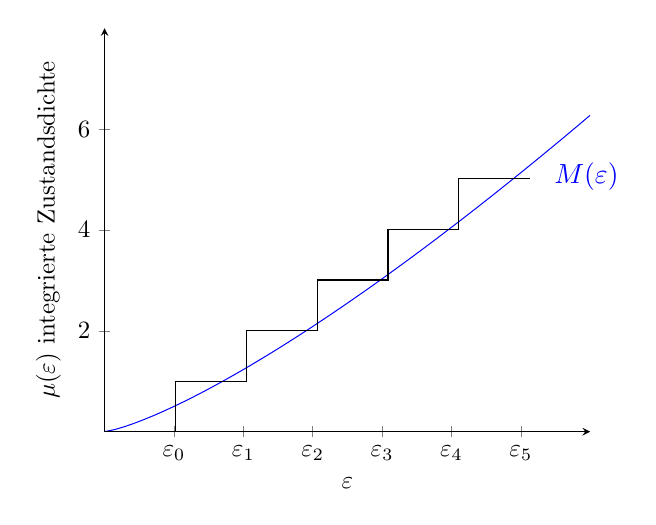
\begin{tikzpicture}[scale=0.9]
        \begin{axis}[
        axis lines = left,
        xmin=0, xmax=7,
        ymin=0, ymax=8,
        xlabel={$\varepsilon$},
        ylabel={$\mu(\varepsilon)$ integrierte Zustandsdichte},
        xtick={1,2,3,4,5,6},
        ytick={2,4,6},
        xticklabels={$\varepsilon_0$,$\varepsilon_1$,$\varepsilon_2$, $\varepsilon_3$,$\varepsilon_4$,$\varepsilon_5$}
        ]
        \addplot[color=blue,samples=50,domain=0:7]{0.5*x^(1.3)};
        \end{axis}
        \draw (0,0) -- (1,0) -- (1,0.713) -- (2,0.713) -- (2,1.426) -- (3,1.426) -- (3,2.14) -- (4,2.14) -- (4,2.853) -- (5,2.853) -- (5,3.566) -- (6,3.566);
        \draw[blue] (6.8,3.6) node{$\Bar{M}(\varepsilon)$};
    \end{tikzpicture}
\end{center}

Im folgenden Querstrich $\Bar{d}$ wird weggelassen

\begin{beispiel}{Bsp}
    \begin{align}
        N &= \int d\varepsilon \ d(\varepsilon) n_\varepsilon \\
        n_\varepsilon &= \frac{1}{e^{\beta (\varepsilon-\mu)}} \pm 1\\
        U &= \int d\varepsilon \ d(\varepsilon) \ \varepsilon \ n_\varepsilon 
    \end{align}
    
     Nutze Energie-Impuls-Relation $\varepsilon(p)$:

     \begin{itemize}
         \item \textbf{Freies Teilchen} 
         \begin{equation}
             \varepsilon (p) = \sqrt{m^2c^4+ c^2p^2} = \begin{cases}
                 mc^2+\frac{p^2}{2m} \ , \frac{p}{m} \ll c \text{  nicht relativistisch}\\
                 cp \ , \text{ mit } m=0 \text{ hochrelativistischer Grenzfall (Photonen)}
             \end{cases}
         \end{equation}
         \item  andere $\varepsilon(p) , z.b. Phononen$
     \end{itemize}
\end{beispiel}

\begin{beispiel}{1 Teilchen in 3D-Volumen mit Spin $s$ und Dispersion $\varepsilon(p) = \frac{p^2}{2m}$}
    Zustandsdichte
    \begin{align}
        d(\varepsilon) & = \sum_k \delta(\varepsilon-\varepsilon_k) = (2s+1) \frac{V}{h^3} \ 4\pi \int_0^\infty dp \ p^2 \ \underbrace{\delta(\varepsilon-\varepsilon_l) }_{\delta(p-\sqrt{2m\varepsilon}) \frac{m}{p}}\\
      \Rightarrow \ d(\varepsilon)  &= (2s+1) 4\pi \sqrt{2} \ \frac{V m^{3/2}}{h^3} \sqrt{\varepsilon} \ \Theta(\varepsilon)
    \end{align}
        
  \textbf{Bem.:} abhängig von Dimension und Dispersion $\varepsilon(p)$. Sei $\varepsilon(p) = \frac{p^2}{2m}$ 
    \begin{align}
        d=3 && d(\varepsilon) \sim \varepsilon^{1/2}\\
        d=2 && d(\varepsilon) \sim \varepsilon^{0}\\
        d=1 && d(\varepsilon) \sim \varepsilon^{-1/2}
    \end{align}
\end{beispiel}


\paragraph{Mittlere Teilchenzahl in 3D -Volumen:}
\begin{align}
    N &= \int d\varepsilon \ d(\varepsilon) \ n_\varepsilon = (2s+1)4\pi \sqrt{2} \frac{V m^{3/2}}{h^3} \int_0^\infty d\varepsilon \sqrt{\varepsilon} \underbrace{\frac{1}{e^{\beta (\varepsilon-\mu)} \pm 1}}_{n_\varepsilon} \\
    &\overset{x=p\varepsilon}{=} \frac{V}{\lambda^3} (2s+1)\frac{2}{\sqrt{\pi}} \int dx \frac{x^{1/2}}{e^{x-\beta\mu} \pm 1}\\
    \lambda &:= \frac{h}{\sqrt{2\pi mkT}} \ \text{thermische De-Broglie Wellenlänge}
\end{align}

Klassischer Grenzfall:
 \begin{align}
     n_\varepsilon \ll 1 && \Leftrightarrow && e^{\beta(\varepsilon-\mu) } \gg 1
 \end{align}
\begin{equation}
    N \approx \frac{V}{\lambda^3} \ (2s+1)  \ \underbrace{\frac{2}{\sqrt{\pi}}\  \int_0^\infty dx \ \frac{x^{1/2}}{e^{x-\beta\mu}}}_{\Gamma(1/2 =1}
\end{equation}

\begin{equation}
    \frac{N\lambda^3}{V \, (2s+1)} = e^{\beta \mu} \overset{\varepsilon \approx 0}{\ll} 1
\end{equation}

\begin{equation}
    \Longrightarrow \quad \fcolorbox{green!70!black}{white}{$\lambda \ll \left(\frac{V}{N}\right)^{1/3}$} \qq{klassicher Grenzfall}
\end{equation}

thermische Wellenlänge $\ll$ typischer Abstand  (erfüllt für: kleine Dichte $\frac{N}{V} \rightarrow 0$ , hohe Temperatur $\lambda \rightarrow 0$)

\textbf{Bem.:} Man kann zeigen (nächste Ordnung in Störungstheorie)
\begin{equation}
    \frac{pV}{mkT} = 1 \pm \frac{\lambda^3}{(2s+1) 2^{3/2}} \frac{N}{V} \begin{cases}
        \text{Fermionen}\\ \text{Bosonen}
    \end{cases}
\end{equation}

\begin{itemize}
    \item Fermionen:  höherer Druck $\rightarrow$ effektive Abstoßung
    \item Bosonen:  niedriger Druck $\rightarrow$ effektive Anziehung
\end{itemize}

\subsection{Fermi-Gas}

\begin{align}
    \hat{H} &= \sum_k \varepsilon_k \hat{n}_k \\
    \langle \hat{n}_k \rangle &= \frac{1}{e^{\beta (\varepsilon_k -\mu)} +1} = f(\varepsilon)  \ \text{Fermi-Fkt.}\\
    \hat{N} &= \sum_k\hat{n}_k
\end{align}
\begin{center}
    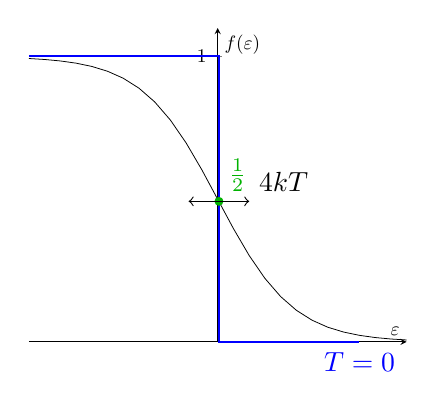
\begin{tikzpicture}[scale=.7]
        \begin{axis}[
        axis lines = center,
        xtick=\empty,
        ytick={0,1},
        ymin=0, ymax=1.1,
        xlabel=$\varepsilon$,
        ylabel=$f(\varepsilon)$
        ]
        \addplot[black]{1/(e^(x)+1)};            
        \end{axis}
        \draw[thick, blue](0,5.18) -- (3.45,5.18) -- (3.45,0) -- (6,0) node[anchor=north]{$T=0$};
        \filldraw[green!70!black] (3.45,2.55) circle (2pt) node[anchor=south west]{$\frac{1}{2}$};
        \draw[<->] (2.9,2.55) -- (4,2.55) node[anchor=south west]{$4kT$};
    \end{tikzpicture}
\end{center}
Ableitung bei $\varepsilon-\mu$:
\begin{equation}
    \abl{f(\varepsilon)}{\varepsilon}\bigg|_{\varepsilon=\mu} =  - \frac{e^{\beta (\varepsilon-\mu)} \beta}{\left( e^{\beta (\varepsilon-\mu)} +1 \right)^2} \bigg|_{\varepsilon=\mu} = -\frac{\beta}{4} =-\frac{1}{4kt}
\end{equation}

Symmetrie:
\begin{align}
    f(\varepsilon) &= \frac{1}{2} - \frac{1}{L} \tanh \left( \frac{\varepsilon-\mu}{2kT} \right) \\
    f(\varepsilon) &\overset{T\to 0}{\longrightarrow }\Theta(\varepsilon-\mu)
\end{align}
\begin{multicols}
    {} Fermi-Energie $\varepsilon_F$ ist definiert für $T=0$. $\varepsilon_F$ zwischen höchster besetzter und niedrigster unbesetzter Einteilchenenergie. Bei $T=0$ ist $\mu = \varepsilon_F$.
    \begin{center}
    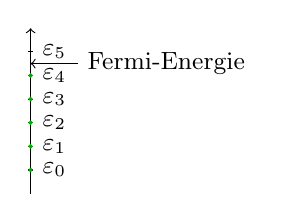
\begin{tikzpicture}[scale=0.3]
      \draw[->] (0,0) -- (0,7);
      \draw (-0.1,1) -- (0.1,1) node[anchor=west]{\small$\varepsilon_0$};
      \draw (-0.1,2) -- (0.1,2) node[anchor=west]{\small$\varepsilon_1$};
      \draw (-0.1,3) -- (0.1,3) node[anchor=west]{\small$\varepsilon_2$};
      \draw (-0.1,4) -- (0.1,4) node[anchor=west]{\small$\varepsilon_3$};
      \draw (-0.1,5) -- (0.1,5) node[anchor=west]{\small$\varepsilon_4$};
      \draw (-0.1,6) -- (0.1,6) node[anchor=west]{\small$\varepsilon_5$};
      \filldraw[green!70!black] (0,1) circle (2pt);
      \filldraw[green!70!black] (0,2) circle (2pt);
      \filldraw[green!70!black] (0,3) circle (2pt);
      \filldraw[green!70!black] (0,4) circle (2pt);
      \filldraw[green!70!black] (0,5) circle (2pt);
      \draw[<-] (0,5.5) -- (2,5.5) node[anchor=west]{\small Fermi-Energie};
    \end{tikzpicture}
    \end{center}
\end{multicols}

Fermi-Temperatur
\begin{equation}
    \theta_F := \frac{\varepsilon_F}{k}\begin{cases}
        T\ll \theta_F \ \text{entartetes Quantengas}\\ T\gg \theta_F \ \text{klass. Grenzfall  } \lambda \ll \left( \frac{V}{N}\right)^{1/3}
    \end{cases}
\end{equation}

\begin{beispiel}{Bsp. Fermionen im 3D-Volumen bei $T \to 0$}
\begin{align}
    N(T=0)&= \int_0^{\varepsilon_F} d\varepsilon\ d(\varepsilon) \\
    d(\varepsilon) &\sim \frac{(2s+1) V\, m^{3/2}}{h^3} \ \sqrt{\varepsilon} \\
    \Rightarrow \ \varepsilon_F &\sim \left(\frac{N}{V}\right)^{2/3}
\end{align}

\begin{equation}
    \left(E_\text{kin} = \varepsilon_F \sim \left(\frac{N}{V} \right)^{2/3}, \ \ E-\text{Coulomb} \sim \frac{1}{r} \sim \left(\frac{N}{V}\right)^{1/3} \right)
\end{equation}
 Energie pro Teilchen:
 \begin{equation}
     \frac{U}{N} = \frac{\int_{-\infty}^{\varepsilon_F} d\varepsilon \ \varepsilon \  d(\varepsilon)}{\int_{-\infty}^{\varepsilon_F} d\varepsilon \  d(\varepsilon)} = \frac{\int_{0}^{\varepsilon_F} d\varepsilon \ \varepsilon^{3/2}}{\int_{0}^{\varepsilon_F} d\varepsilon \  \varepsilon^{1/2}} = \frac{3}{5 } \varepsilon_F
 \end{equation}


    Fermi-Druck

    \begin{equation}
        p \sim \left( \frac{N}{V}\right) ^{5/3}
    \end{equation}
\end{beispiel}

\subsubsection{Tiefe Temperaturen $ T\ll \Theta_F=: \frac{\varepsilon_F}{k}$}

Ziel: Wärmekapazität $C_V$
\begin{equation}
    c_V = \left({\frac{\partial U}{\partial T}}\right)_{V,N} \ \text{z.B. Metallelektronen}
\end{equation}
\begin{itemize}
    \item[Problem:] Großkanonisches Ensemble hat kein festes $N$
    \item[Lösung:] im thermodynamischen Limes gilt: $\underbrace{\expval{N}}_{\text{großkan.}} = \underbrace{N}_{\text{kan}}$
    \begin{enumerate}
    \item Bestimme $N(T,V,\mu) \quad \Rightarrow \quad \mu(T,V,N)$
    \item Bestimme $U(T,V,\mu) \quad \stackrel{\text{elimin. } \mu}{\Longrightarrow}\quad U(T,V,N)$
    \item $C_V$
    \end{enumerate} 
\end{itemize}

\paragraph{1a)} Bestimme $N(T,V,\mu)$ im großkanonischen Ensemble
\begin{itemize}
    \item[$T>0$:] Zustände oberhalb von $\mu$ besetzt
    \item[] Zustände unterhalb von $\mu$ geleert
    \begin{center}
        \begin{tikzpicture}
            \draw[thick,->] (0,-0.1) -- (0,3) node[anchor=south east]{$f(\varepsilon)$};
            \draw[thick,->] (-0.1,0) -- (8,0) node[anchor=west]{$\varepsilon$};
            \draw (3,2.9) -- (-0.1,2.9) node[anchor=east]{1};
            \draw (3,2.9) -- (3,-0.1) node[anchor=north]{$\mu$};
            \draw[green!70!black] plot [smooth] coordinates{(0,2.9) (2,2.61) (3,1.45) (4,0.29) (8,0.1)};
            \draw (3.2,3.3) node{$T=\SI{0}{\K}$};
            \draw[green!70!black] (6,1) node{$T>0$};
        \end{tikzpicture}
    \end{center}
    \item[] Zustandsdichte $d(\varepsilon)$ steigt i.A.
    \begin{itemize}
        \item[$\Rightarrow$] mehr Zustände oberhalb von $\mu$
        \begin{center}
        \begin{tikzpicture}
            \draw[thick,->] (0,-0.1) -- (0,3) node[anchor=south east]{$d(\varepsilon)$};
            \draw[thick,->] (-0.1,0) -- (6,0) node[anchor=west]{$\varepsilon$};
            \draw[thick] (3,0.1) -- (3,-0.1) node[anchor=north]{$\mu$};
            \draw[blue] plot [smooth] coordinates{(2,1.5) (3,2.4) (4,2.8)};
        \end{tikzpicture}
    \end{center}
        \item[] großkan.: $N(T)$ wächst, $\mu = const.$
        \item[] kan.: $N=const.$, $\mu(T)$ sinkt
    \end{itemize}
\end{itemize}
\subparagraph{Sommerfeld-Entwicklung}
\begin{align}
    N(T,\mu) = \int_{-\infty}^{\infty} d\varepsilon \ d(\varepsilon) \ f(\varepsilon) &= \int_{-\infty}^{\infty} d\varepsilon \ d(\varepsilon) \ \underbrace{f_{T=0}(\varepsilon)}_{=\theta(\mu-\varepsilon)} + \int_{-\infty}^{\infty} d\varepsilon \ d(\varepsilon) \underbrace{\left[ f(\varepsilon) - f_{T=0}(\varepsilon)\right]}_{*}\\
    &= \underbrace{\int_{-\infty}^{\mu} d\varepsilon \ d(\varepsilon)}_{=N(T=0,\mu)} + \int_{-\infty}^{\infty} d\varepsilon \ d(\varepsilon) \left[ f(\varepsilon) - f_{T=0}(\varepsilon)\right]
\end{align}
\begin{itemize}
    \item[$\rightarrow$] zu (*):
    \begin{center}
        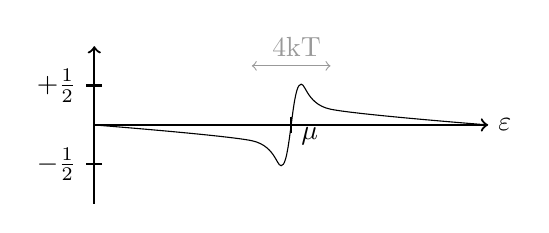
\begin{tikzpicture}
            \draw[thick,->] (0,-1) -- (0,1);
            \draw[thick,->] (0,0) -- (5,0) node[anchor=west]{$\varepsilon$};
            \draw[thick] (0.1,0.5) -- (-0.1,0.5) node[anchor=east]{$+\frac{1}{2}$};
            \draw[thick] (0.1,-0.5) -- (-0.1,-0.5) node[anchor=east]{$-\frac{1}{2}$};
            \draw[thick] (2.5,-0.1) -- (2.5,0.1) node[anchor=north west]{$\mu$};
            \draw plot [smooth] coordinates{(0,0) (2,-0.2) (2.4,-0.5) (2.6,0.5) (3,0.2) (5,0)};
            \draw[black!40,<->] (2,0.75) -- (3,0.75) node[anchor=south east]{4kT};
        \end{tikzpicture}
    \end{center}
    \item[$\rightarrow$] Entwicklung der Zustandsdichte: $d(\varepsilon) = d(\mu) + d^{\prime}(\mu) \cdot (\varepsilon - \mu) + o(\varepsilon^2)$
\end{itemize}

\begin{align}
    N(T,\mu) &= N(T=0,\mu) + d(\mu) \underbrace{\int_{-\infty}^{\infty} d\varepsilon \ [ \underbrace{f(\varepsilon) - f_{T=0}(\varepsilon)}_{\text{ungerade Fkt.}}]}_{=0} + d^{\prime}(\mu) \int_{-\infty}^{\infty} d\varepsilon \ \underbrace{(\varepsilon - \mu) \left[ f(\varepsilon) - f_{T=0}(\varepsilon)\right]}_{\text{gerade Fkt}} + ...\\
    &= N(T=0,\mu) + d^{\prime}(\mu) \cdot \underbrace{2 \cdot \int_{\mu}^{\infty} d\varepsilon \ (\varepsilon - \mu) [ f(\varepsilon) - \underbrace{f_{T=0}(\varepsilon)}_{=0 \text{ für } \varepsilon>\mu}]}_{\stackrel{x = \beta(\varepsilon-\mu)}{=} 2 \cdot (kT)^2 \int_0^{\infty} dx \ \frac{x}{e^x+1} = \frac{1}{2} \zeta(2) = \frac{1}{2} \frac{\pi^2}{6}} + ...
\end{align}

\begin{prop}{Häufige Integrale für Fermi- und Bosegase}
    \begin{align}
        &\int_0^\infty dx \ \frac{x^{t-1}}{e^x +1} = \left(1-\frac{1}{2^{t-1}}\right) \Gamma(t) \zeta(t) \\
        &\int_0^\infty dx \ \frac{x^{t-1}}{e^x -1} =  \Gamma(t) \zeta(t)
    \end{align}
    mit Riemannscher Zeta-Funktion:
    \begin{equation}
        \zeta(t) = \sum_{n=1}^\infty \frac{1}{n^t}
    \end{equation}
\end{prop}
\begin{equation}
    N(T,\mu) = N(T=0,\mu) + \frac{\pi^2}{6}(kT)^2 \, d^{\prime}(\mu) + o((kT)^4)
\end{equation}

\paragraph{1b)} Bestimme $\mu (T)$ bei festem $V,N$:
\begin{align}
    N(T,\mu(T))&= \underbrace{N(T=0,\mu(T))}_{*} + \frac{\pi^2}{6} (k)^2 d^\prime(\mu(T)) + ...\\
    * &=\int_{-\infty}^{\mu(T)} d\varepsilon \ d(\varepsilon) = \underbrace{\int_{-\infty}^{\varepsilon_F} d\varepsilon \ d(\varepsilon)}_{N} + \underbrace{\int_{\varepsilon_F}^{\mu(T)} d\varepsilon \ d(\varepsilon)}_{(\mu(T)-\varepsilon_F) d(\varepsilon_F)}\\
    \Rightarrow \ \ \mu(T)&= \varepsilon_F - \frac{\pi^2}{6} (kT)^2 \frac{d^\prime(\varepsilon_F)}{d(\varepsilon_F)} + o\left( (8kT)^4 \right)
\end{align}

\paragraph{2} ...
\begin{equation}
    U(T) = U(\varepsilon_F) + \frac{\pi^2}{6} \, (kT)^2 \, d(\varepsilon_F) + o\left((kT)^4 \right)
\end{equation}

\paragraph{3}
\begin{equation}
    C_V = \left( \pdv{U}{T} \right)_{V,N} \propto T
\end{equation}
Phononen: $C_V \propto T^3$ \\
Dulong-Petit: $C_V \propto T^0$
\begin{center}
    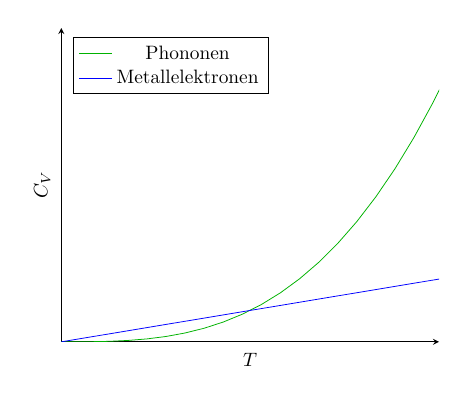
\begin{tikzpicture}[scale=0.7]
        \begin{axis}[axis lines= left,
        ylabel = $C_V$,
        xlabel = $T$,
        xmin = 0 , xmax = 2,
        ymin=0, ymax = 10,
        xtick=\empty,
        ytick=\empty,
        legend pos=north west,]
        \addplot[green!70!black,samples=100]{x^3};
        \addlegendentry{Phononen},
        \addplot[blue,samples=100]{x};
        \addlegendentry{Metallelektronen};
            
        \end{axis}
    \end{tikzpicture}
\end{center}


\subsection{Bose-Einstein-Kondensation} \marginpar{VL 22}
Bose-Gas mit fester Teilchenzahl $N$\\
Problem: Formel Großkanonisches Ensemble\\
Lösung:\\
Bestimme $\mu(T,\frac{N}{V})$ aus
\begin{align}
    N \overset{th. Lim.}{=} \expval{N} = \sum_k \expval{n_k} = \sum_k \frac{1}{e^{\beta(\varepsilon_k-\mu)}-1}
\end{align}
Bem.:
\begin{align}
    \forall k: \space 0 \leq \expval{n_k} \Leftrightarrow \forall k: \mu < \varepsilon_k \rightarrow \mu < \min_k \varepsilon_k= \varepsilon_0 
\end{align}
System idealer Bosonen in 3D Volumen, nicht relativistisch: $\varepsilon(p)=\frac{p^2}{2m}$\\
Zustandsdichte:
\begin{align}
    d(\varepsilon)=(2s+1) \ 4\pi \sqrt{2} \ \frac{Vm^{\frac{3}{2}}}{h^3} \sqrt{\varepsilon} \ \Theta(\varepsilon) \sim \sqrt{\varepsilon}
\end{align}
period. Randbed. $\Rightarrow \ \varepsilon_0=0$\\
Besetzung Grundzustand :
\begin{align}
    \expval{n_0} \stackrel{\mu=-kT}{=} \frac{1}{e-1} = 0,58
\end{align}
Teilchenzahl
\begin{align}
    N &= \sum_k \frac{1}{e^{\beta(\varepsilon_k-\mu)}-1}
    =\int_0^{\infty} d\varepsilon \ d(\varepsilon) \frac{1}{e^{\beta(\varepsilon_k-\mu)}-1}\\
    &\overset{x=\beta\varepsilon}{=} (2s+1) \frac{2}{\sqrt{\pi}}\frac{V}{\lambda^3} I(z)
    \label{eq:BEK}
\end{align}
\begin{itemize}
    \item exakt: wenn $d(\varepsilon) = \sum_k \delta(\varepsilon-\varepsilon_k)$
    \item Näherung: wenn geglättetes $\Bar{d}(\varepsilon) \propto \sqrt{\varepsilon}$
\end{itemize}
\begin{align}
    \text{mit } \lambda=\frac{h}{\sqrt{2\pi mkt}}, \quad I(z) = \int_0^{\infty} dx \ \frac{\sqrt{x}}{\frac{e^x}{z}-1}\\
    \text{außerdem } z=e^{\beta \mu} \ \text{(Fugazität) mit } \mu < 0 \Rightarrow z\in [0,1[
\end{align}
Wie sieht $I(z)$ aus?
\begin{align}
    I(z)= \Gamma\left(\frac{3}{2}\right) Li_{\frac{3}{2}}(z) \text{ mit polylog. } Li_S(z)=\sum_{n=1}^\infty \frac{z^n}{n^S}
\end{align}
Maximalwert bei $z=1$:
\begin{align}
    Li_S(z)=\zeta(S) \ \Rightarrow I(z=1)=\Gamma\left(\frac{3}{2}\right) \zeta\left(\frac{3}{2}\right) \approx 2,3
\end{align}
\begin{center}
    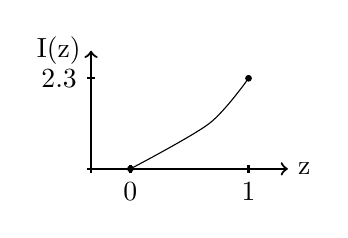
\begin{tikzpicture}[scale=0.5]
        \draw[thick,->] (-0.1,0) -- (5,0) node[anchor=west]{z};
        \draw[thick,->] (0,-0.1) -- (0,3) node[anchor=east]{I(z)};
        \draw[thick] (0.1,2.3) -- (-0.1,2.3) node[anchor=east]{2.3};
        \draw[thick] (1,0.1) -- (1,-0.1) node[anchor=north]{0};
        \draw[thick] (4,0.1) -- (4,-0.1) node[anchor=north]{1};
        \draw plot [smooth] coordinates{(1,0) (3,1.15) (4,2.3)};
        \filldraw (1,0) circle (2pt);
        \filldraw (4,2.3) circle (2pt);
    \end{tikzpicture}
\end{center}
$\Rightarrow$ maximale Teilchenzahl im Limes $\mu \rightarrow 0^- \ (z \rightarrow 1)$
\begin{align}
    N_c(T,V) = (2s+1) \ \zeta\left(\frac{3}{2}\right) \frac{V}{\lambda^3}
\end{align}
Bem.:\\
Dieses $N_c$ entspricht  (bis auf Faktoren) dem Übergang:\\
\begin{center}
    \begin{tabular}{ccc}
    klass. Grenzfall & $\longleftrightarrow$ & Quantengas\\
    $N << N_c$ &  & $N \overset{\approx}{>} N_c$\\
\end{tabular}
\end{center}

$\Rightarrow$ kritische de-Broglie Wellenlänge
\begin{align}
    \lambda_c\left(\frac{N}{V}\right) = \left((2s+1) \zeta\left(\frac{3}{2}\right) \frac{V}{N}\right)^{\frac{1}{3}}
\end{align}
$\Rightarrow$ kritische Temperatur $T_c$ (Bose-Temp.)
\begin{align}
    T_c\left(\frac{N}{V}\right) = \frac{h^3}{2\pi mk} \left((2s+1) \zeta\left(\frac{3}{2}\right) \frac{V}{N}\right)^{-\frac{2}{3}}
\end{align}
Bem.: eliminiere $V$ $\frac{N}{N_C}=\left(\frac{T}{T_C}\right)^{\frac{3}{2}}$ (für später)\\
Für $N>N_c$ oder $T< T_c$ gibt es kein $\mu,z$, so dass \ref{eq:BEK} erfüllt ist.\\
Eigenschaften von:
\begin{align}
    N = \sum_k \frac{1}{e^{\beta(\varepsilon_k-\mu)}-1} = \sum_k \frac{1}{\frac{e^{\beta \varepsilon_k}}{z}-1}
\end{align}
\begin{itemize}
    \item alle Terme $>0$
    \item Terme monoton abfallend für wachsende  $\varepsilon_k$
    \item Größter Beitrag individueller Beitrag für $ \varepsilon_0$ (hier $\varepsilon_0=0$)
        \begin{align}
            \expval{n_0}=\frac{1}{\frac{1}{z}-1}= \frac{z}{1-z} \ \overset{z \rightarrow 1}{\rightarrow} \infty
        \end{align}
        \begin{itemize}
            \item beliebig groß. makroskopische Werte $O(N)$ möglich !
            \item dieser Beitrag fehlt im Integral, da $\Bar{d}(\varepsilon=0)=0$
        \end{itemize}
    \item Man kann zeigen, weitere individuelle Beiträge $\expval{n_k} << \expval{n_0}$
\end{itemize}
\begin{align}
    \Rightarrow N= \sum_k \frac{1}{e^{\beta(\varepsilon_k-\mu)}-1} = \expval{n_0} + \int_0^\infty d\varepsilon \ d(\varepsilon) \frac{1}{e^{\beta(\varepsilon-\mu)}-1}
\end{align}
Für $T<T_c$ ist $\expval{n_0}=N-N_c= O(N)$ makroskopisch\\
\begin{align}
    &\Rightarrow \expval{n_0} = \frac{1}{e^{-\beta\mu)}-1} \approx -\frac{1}{\beta\mu}\\
    &\Rightarrow \mu \approx -\frac{kT}{\expval{n_0}} \text{ ist extrem klein}\\
    &\Rightarrow \mu \to 0 \qq{bzw.} z \to 1
\end{align}
$\Rightarrow$ Im Integral $\mu = 0$ setzen $\Rightarrow$ $z=1$
\begin{align}
    \fcolorbox{red}{white}{\large$N=\expval{n_0} + N_c(T,V)$}
\end{align}
\begin{itemize}
\item[]$T= const$: $N>N_C$ werde erhöht $\Rightarrow$ alle weiteren Bosonen gehen in den Grundzustand, exp. wichtiger:
\item[]$N=const$: $T<T_c$ werdem erniedrigt $\Rightarrow$ $N_c=N\left(\frac{T}{k}\right)^{\frac{3}{2}}$ sinkt $\Rightarrow$ $\expval{n_0}$ wächst
\begin{align}
    \expval{n_0}=N-N_c = N\left[1-\left(\frac{T}{T_c}\right)^{\frac{3}{2}}\right]
\end{align}
\end{itemize}
\begin{center}
    \begin{tikzpicture}[scale=0.6]
        \begin{axis}[
        axis lines = left,
        ylabel={$\frac{\expval{n_0}}{N}$},
        xlabel={$\frac{T}{T_C}$},
        ytick={1},
        xtick={1},
        xmin=0, xmax=1.5,
        ymin=0, ymax=1.2,
        ]
        \addplot[domain=0:1]{1-x^(3/2)};
        \addplot[blue,domain=0:1]{x^(3/2)};
        \addplot[blue,domain=1:1.5]{1};
        \end{axis}
        \draw[blue] (3,5) node[anchor=west]{\tiny Teilchen im angeregten Zustand};
    \end{tikzpicture}
\end{center}
\begin{definition}{Bose-Einstein-Kondensation}
    makroskopisches Quantenphänomen,
    Phasenübergang: bei $T<T_c$ existieren 2 Phasen
    \begin{itemize}
        \item $\expval{n_0}$ Teilchen im Grundzustand
        \item $N-\expval{n_0}$ Teilchen im angeregten Zuständen
        \item Phasen räumlich nicht getrennt (nur bei flüssig/gasförmig)
    \end{itemize}
\end{definition}
\textbf{Bem.:} Wenn $T$ klein genug $\Rightarrow$ alle Teilchen im Grundzustand nach klass. Maxwell-Boltzmann-Statistik
\begin{align}
    \frac{\expval{n_0}}{\expval{n_1}} = \frac{e^{-\beta \varepsilon_0}}{e^{-\beta \varepsilon_1}}=e^{\beta(\varepsilon_1-\varepsilon_0)} >> 1 \text{ für kleine }T
\end{align}
Bei welchen T?
\begin{align}
    kT << \varepsilon_1-\varepsilon_0 = \frac{\hbar^2(\Delta k)^2}{2m} = \frac{\hbar^2}{2m}\left(\frac{2\pi}{L}\right)^2 = \frac{\hbar^2}{2m}\left(\frac{1}{V}\right)^{\frac{2}{3}} \widehat{=} \lambda \gg V^{\frac{1}{3}}
\end{align}
Zum Vergleich $T_c$ BEC:
\begin{align}
    kT_c = \frac{\hbar^2}{m}\left(\frac{N}{V}\right)^{\frac{2}{3}} \widehat{=} \lambda \approx V^{\frac{1}{3}}
\end{align}
$\Rightarrow$ BEC bereits bei um $N^{\frac{2}{3}}$ höheren Temperaturen \\
Ursache: Bose-Einstein-Statistik für identische quantenmechanische Teilchen

\paragraph{Experiment:}
\begin{itemize}
    \item Problem: hier nur ideales Bose-Gas, real: WW
    \item verbundene Phänomene:
    \begin{itemize}
        \item Supraleitung (Cooper-Paare)
        \item Superfluidität ($^4 He$)
    \end{itemize}
    \item[$\Rightarrow$] experimentelle Umsetzung: weniger WW $\rightarrow$ Gas
    \begin{itemize}
        \item niedrige Temperatur $\rightarrow$ Verflüssigung
        \begin{itemize}
            \item[$\Rightarrow$] Lösung: verdünntes Gas 
        \end{itemize}
    \end{itemize}
    \item[$\Rightarrow$] erstmals 1995 gelungen, 2001 Nobelpreis
    \item[$\Rightarrow$] $10^{-6} \si{\K} = T$ notwendig
\end{itemize}

\subsection{Photonengas}\marginpar{VL 23}
\begin{wrapfigure}{l}{0.2\textwidth}
   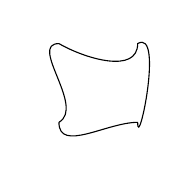
\begin{tikzpicture}
    \coordinate (x1) at (0,0);
    \coordinate (x2) at (1,0);
    \coordinate (y1) at (0,1);
    \coordinate (y2) at (1,1);
    \draw (x1) to[out=-90,in=-180] (x2) to[out=-90,in=30] (y2) to[out=-90,in=-30] (y1) to[out=180,in=30] (x1);
\end{tikzpicture} 
\end{wrapfigure}
Elektromagnetische Strahlung im Gleichgewicht mit Hohlraumwand \\ $\Rightarrow$ Maxwell Gleichungen $\rightarrow$ lineare Superposition von monochromatischen Eigenzuständen. \\ Eigenmoden:
\begin{itemize}
    \item durch Form und Randbedingungen festgelegt
    \item sehen i.A. irregulär aus
    \item hier nur mittlere Dichte der Eigenfrequenzen wichtig
\end{itemize}
Zustandsdichte (siehe \cref{abs.Kontinuumslimes})
\begin{itemize}
    \item in $k = \abs{\Vec{k}}$:
    \begin{equation}
        d(k) = \underbrace{2}_{\substack{Maxwell-Gl: \\ \Vec{E},\Vec{B} \perp \Vec{k}}} \cdot \left(\frac{L}{2\pi}\right)^3 \cdot \underbrace{\overbrace{4\pi k^2}^{\text{\tiny Oberfläche}} \cdot dk}_{\text{\tiny Kugelschale}} = \frac{V}{\pi^2} k^2 \, dk
    \end{equation}
    \item in $\omega = ck$:
    \begin{equation}
        d(\omega) \, d\omega = \frac{V}{\pi^2c^3} \omega^2 \, d\omega
    \end{equation}
    \item in $\varepsilon=\hbar \omega$:
    \begin{equation}
        d(\varepsilon) \, d\varepsilon = \frac{V}{\pi^2\hbar^3c^3} \varepsilon^2\, d\varepsilon
    \end{equation}
    \item[] \color{black!40} Man nutzt hier die Multipikation mit dem Differential, um eine dimensionslose Größe zu erzeugen und damit die Ausdrücke auf der linken Seite gleichsetzen zu können. Es gilt dann:
    \begin{equation}
         d(x) \, dx = d(x(y)) \dv{x}{y} \, dy
    \end{equation}
    \begin{itemize}\color{black}
        \item[$\rightarrow$] klassische ED: Amplitude der Eigenmode $k$ kontinuierlich
        \item[] QED: Qunatisierung der mode analog zum H.O.:
        \begin{align}
            \varepsilon_n &= \hbar \omega(k) \left(\frac{1}{2}+n\right) \qquad n=0,1,2,...\\
            &\Rightarrow n \qq{Photonen (Bosonen) im Einteilchenzustand mit Energie $\hbar \omega$}
        \end{align}
    \end{itemize}
\end{itemize}

\paragraph{statistiscche Eigenschaften der Photonen} (wichtig für Besetzung $n_k$)
\begin{itemize}
    \item Spin = 1 $\Rightarrow$ Bosonen
    \item keine WW $\Rightarrow$ ideales Bosegas
    \item ABER: Anzahl der Photonen ist keine Erhaltungsgröße (ständige Absorption/Emission der Photonen an Wand)
    \begin{equation}
        \varrho = \frac{1}{Z} e^{-\beta H} \qq{mit beliebiger Teilchenzahl}
    \end{equation}
    \begin{itemize}
        \item[] vgl. mit großkanonischem Ensemble: \fcolorbox{green!70!black}{white}{$\mu = 0$} für Photonen
        \begin{equation}
            \Rightarrow \qq{mittlere Besetzungszahl:} \expval{n_k} = \frac{1}{e^{\beta \varepsilon_k}-1}
        \end{equation}
    \end{itemize}
\end{itemize}

\subsubsection{Planck'sches Strahlungsgesetz}
\begin{equation*}
    \qq{spektrale Energiedichte} = \frac{\text{Energie}}{\text{Volumen}\cdot \text{Energieintervall}}
\end{equation*}
\begin{align}
    \varrho(\varepsilon,T) \, d\varepsilon &= \frac{1}{V} \cdot d(\varepsilon) \cdot \expval{n_{\varepsilon}} \cdot \varepsilon \, d\varepsilon\\
    &= \frac{1}{V} \cdot \frac{V}{\pi^2\hbar^3c^3}\varepsilon^2 \cdot \frac{1}{e^{\beta\varepsilon}-1}\cdot \varepsilon \, d\varepsilon\\
    &= \frac{\varepsilon^3 \, d\varepsilon}{\pi^2\hbar^3c^3\left(e^{\beta \varepsilon}-1\right)}
\end{align}
in $\omega\quad(\varepsilon=\hbar\omega)$:
\begin{align}
    \fcolorbox{red}{white}{$\varrho(\omega,T) \, d\omega = \frac{\hbar}{\pi^2c^3}\frac{\omega^3}{e^{\frac{\hbar\omega}{kT}}-1}\,d\omega$} \quad \text{Planck'sches Strahlungsgesetz (1900)}
\end{align}

\begin{center}
    \begin{tikzpicture}
        \begin{axis}[
        axis lines=left,
        xlabel={$\omega$},
        ylabel={$\varrho(\omega)$},
        xmin=0, xmax=0.5,
        ymin=0, ymax=5.5,
        xtick=\empty,
        ytick=\empty,
        ]
        \addplot[color=blue, samples=100,domain=0:0.5]{100000*(x^3)/(e^(30*x)-1)};
        \addplot[color=red, samples=100,domain=0:0.5]{100000*(x^3)/(e^(40*x)-1)};
        \end{axis}
        \draw[->] (0.75,1) -- (1.25,3) node[anchor=south west]{T};
    \end{tikzpicture}
\end{center}
\begin{itemize}
\item dimensionslos:
\begin{align}
    x &= \frac{\hbar\omega}{kT} \qquad \Tilde{\varrho}:= \varrho \frac{1}{kT} \left(\frac{\hbar c}{kT}\right)^3\\
    &\Rightarrow \Tilde{\varrho}(x) \, dx = \frac{1}{\pi^2} \frac{x^3}{e^x-1} \, dx
\end{align}
\item[]$\rightarrow$ Daraus ist erkennbar, dass es sich im Diagramm oben um die gleichen Kurven handelt, diese lediglich anders skalieren:
\begin{equation*}
    \omega \rightarrow \frac{\omega}{T} \qq{,} \varrho \rightarrow \frac{\varrho}{T^3}
\end{equation*}
\item Maximum:
\begin{equation}
    \dv{\varrho(\omega,T)}{\omega}\stackrel{!}{=} 0 \quad \Rightarrow \quad \omega_{\text{max}} \approx 2.82 \frac{kT}{\hbar} \propto T \qq{(Wien'sches Verschiebungsgesetz)}
\end{equation}
\item Grenzfälle:
\begin{itemize}
    \item $\hbar\omega \ll kT$:
    \begin{equation}
        \varrho(\omega,T) \approx \frac{\omega^2kT}{\pi^2c^3} \qq{(Rayleigh-Jeans-Gesetz)}
    \end{equation}
    \item $\hbar\omega \gg kT$:
    \begin{equation}
        \varrho(\omega,T) \approx \frac{\hbar\omega^3}{\pi^2c^3} e^{-\frac{\hbar\omega}{kT}} \qq{(Wien)}
    \end{equation}
\end{itemize}
\end{itemize}

\paragraph{Energiedichte} $\left(\frac{\text{Energie}}{\text{Volumen}}\right)$
\begin{align}
    u(T) &= \frac{U}{V}= \int_0^{\infty} \varrho(\omega,T) \, d\omega = \frac{\hbar}{\pi^2 c^3}\, \int_0^{\infty} \, d\omega \ \frac{\omega^3}{e^{\frac{\hbar\omega}{kT}}-1}\\
    &\stackrel{x=\frac{\hbar\omega}{kT}}{=} \frac{(kT)^4}{\pi^2c^3\hbar^3} \underbrace{\int_0^{\infty} \, dx \ \frac{x^3}{e^x-1}}_{=\Gamma(4)\zeta(4) = 3! \frac{\pi^4}{90}=\frac{\pi^4}{15}} = \frac{\pi^2(kT)^4}{15 (\hbar c)^3} \propto T^4
\end{align}
\paragraph{Strahlungsdichte} $\left(\frac{\text{Energie}}{\text{Fläche}\cdot\text{Zeit}}\right)$
\begin{center}
\begin{tikzpicture}
    \coordinate (c) at (3,0);
    \draw (c) ellipse (0.5cm and 1cm);
    \draw (c) ellipse (0.3cm and 0.6cm);
    \draw (0,-1)--(0,1);
    \draw[dashed] (0,0)--(c);
    \draw (0,0)--(3,0.6cm);
    \draw (0,0.4cm)--(3,1cm) node[midway,above] {$c dt$};
    \draw[ultra thick, green!50!black] (0,0) -- (0,0.4cm) node[midway, left]{$dA$};
    \draw (3.8,0) node{$\varphi$};
    \draw (1.5,0) arc (0:11:1.5);
    \draw (1,0.1) -- (1,-0.5) node[anchor=north]{$\vartheta$}
\end{tikzpicture}
\end{center}
\begin{align}
    j(T) \,dt\,dA &= u(T) \frac{1}{4\pi} \int_0^{2\pi} \,d\varphi \ \underbrace{\int_0^{\frac{\pi}{2}} \, d\vartheta \ \sin(\vartheta) c \,dt\, \cos(\vartheta)\,dA}_{=\frac{1}{2} c \,dt\,dA} \\
    &\Rightarrow \quad \fcolorbox{red}{white}{$j(T)=\sigma \cdot T^4$} \qq{mit} \sigma = \frac{\pi^2}{60} \frac{k^4}{\hbar^3c^2} \qq{(Stefan-Boltzmann-Gesetz)}
\end{align}

\paragraph{Großkanonisches Potential:}
\begin{align}
    \Phi &= - p \cdot V\\
    \Phi &= -kT \ln(Z_G) = ... = -\frac{V}{3} u(T)
\end{align}
\begin{itemize}
    \item[$\Rightarrow$] Strahlungsdruck:
    \begin{equation}
        p = \frac{1}{3} u(T) \qquad \color{black!40}\left(\text{siehe Übung 12.2: } p = \frac{n}{d}u\right)
    \end{equation}
    \item[$\Rightarrow$] Entropie:
    \begin{align}
        S = - \left(\pdv{\Phi}{T}\right)_{V,\mu} &= \frac{V}{3} \cdot 4 \cdot \frac{u(T)}{T}\\
        &\Rightarrow \quad U = \frac{3}{4} ST
    \end{align}
\end{itemize}

\begin{beispiel}{Beispiel: kosmische Hintergrundstrahlung}
    \begin{itemize}
        \item[] Urknall: Materie und Strahlung im Gleichgewicht
        \item[] $\Rightarrow$ Zeitpunkt der Bildung von Atomen: Trennung von Materie und Strahlung etwa bei Temperatur \SI{3000}{\K}
        \begin{itemize}
            \item[$\rightarrow$] danach: keine Änderung der Verteilung ($\varrho(\omega,T)$) mehr
            \item[$\rightarrow$] Volumen Universum: Faktor 1000
            \item[$\rightarrow$] Temperatur Universum: Faktor $\frac{1}{1000}\quad \Rightarrow$ \SI{3}{\K}
        \end{itemize}
    \end{itemize}
\end{beispiel}



\subsection{Phononengas}\marginpar{VL 24}
Ziel: Beitrag der Gitterschwingungen zur Wärmekapazität von Festkörpern (Metallelektronen $\rightarrow$ Fermi-Gas $\rightarrow$ $C_V\sim T$)\\
\newline
\paragraph{1 D Gitter der Atome:}
\begin{center}
    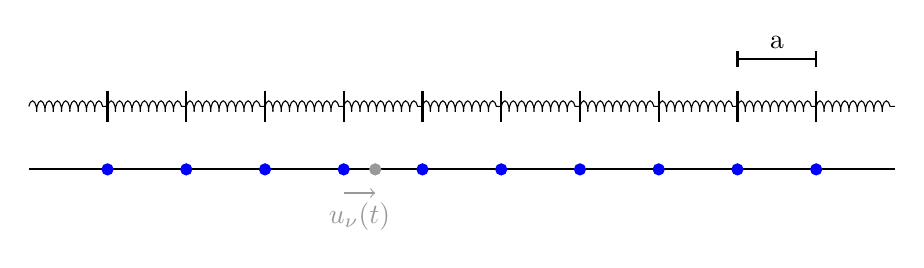
\begin{tikzpicture}
        \draw[thick] (0,0) -- (11,0);
        \foreach \x in {1,2,3,4,5,6,7,8,9,10}{
            \filldraw[blue] (\x,0) circle (2pt);
            \draw[thick] (\x,1) -- (\x,0.6);
        }
        \foreach \x in {1,2,3,4,5,6,7,8,9,10,11}
            \draw[decoration={aspect=0.3, segment length=3pt, amplitude=2pt,coil},decorate] (\x-1,0.8) -- (\x,0.8);
        \draw[thick] (9,1.3) -- (9,1.5);
        \draw[thick] (9,1.4) -- (10,1.4) node[midway,above]{a};
        \draw[thick] (10,1.3) -- (10,1.5);
        \filldraw[black!40] (4.4,0) circle (2pt);
        \draw[->, black!40] (4,-0.3) -- (4.4,-0.3) node[midway,below]{$u_\nu(t)$};
    \end{tikzpicture}
\end{center}
Potentielle Energie:
\begin{align}
    V=V_0+\sum_{\nu =1}^N \frac{K}{2} (u_\nu-u_{\nu+1})^2 \qquad \qquad (\text{per. RB: }U_{N+1}=U_1)
\end{align}
Bewegungsgleichung für Atom j:
\begin{align}
    \ln \pdv[2]{u_j}{t} &= - \pdv{u_j} V = -K(u_j - u_{j+1})-K(u_{j-1}-u_j)\\
    &= -K(2u_j-u_{j+1}-u_{j-1})
\end{align}
N gekoppelte DGL 2.Ordnung
\subparagraph{1. Ansatz Ebene Welle:}
\begin{align}
    u_j^k(t)=Ae^{i(jka-\omega (k) t)}
\end{align}
Einsetzen:
\begin{align}
    -m\omega^2(k)=-K(2-e^{ika}-e^{-ika})=-2K\underbrace{(1-cos(ka))}_{2\sin^2(\frac{ka}{2})}
\end{align}
\begin{align}
    \Rightarrow \ \omega (k) = \underbrace{\pm}_{\text{keine neue Lsg}} 2\sqrt{\frac{K}{m}}\abs{\sin{\frac{ka}{2}}}
\end{align}
reelle Lösung:
\begin{align}
    u_j^k(t)=A\cos{(kja-\omega (k)t)}
\end{align}
erlaubte k-Werte aus RB:
\begin{align}
    u_{N+1}=u_1 \ \Rightarrow e^{ikNa}=1 \ \Rightarrow k=\frac{2\pi n}{aN}, n \in \mathbb{Z}
\end{align}
\begin{align}
    k'=k+\frac{2\pi}{a} \qq{ist eine Lsg}\\
    \Rightarrow \text{wähle }k\in \left[-\frac{\pi}{a},\frac{\pi}{a}\right) \Rightarrow N\text{ Eigenmoden}
\end{align}
Dispersionsrelation:
\begin{center}
    \begin{tikzpicture}[scale=0.8]
        \begin{axis}[
        axis x line=center,
        axis y line=center,
        xlabel= $k$,
        ylabel=$\omega(k)$,
        xmin=-3.2,xmax=3.2,
        ymin=0,ymax=1.1,
        xtick={-3.14,3.14},
        ytick={1},
        xticklabels={$-\frac{\pi}{a}$, $\frac{\pi}{a}$}
        ]
        \addplot[color=blue, samples=100, domain=0:3.141]{sin(deg(x/2))};
        \addplot[color=blue, samples=100, domain=-3.141:0]{-sin(deg(x/2))};
        \end{axis}
    \end{tikzpicture}
\end{center}
$\abs{k}<<\frac{\pi}{a}$:
\begin{align}
    \omega (k)= 2\sqrt{\frac{K}{m}}\abs{\frac{ka}{2}} = \underbrace{\sqrt{\frac{K}{m}} a}_{=c_s \text{ Schallgeschw.(akustische Mode)}} \abs{k}
\end{align}

\subparagraph{2. Ansatz Normalkoordinaten:}
\begin{align}
    \xi^k(t):=\sum_{j=1}^Ne^{-ikja} u_j(t)
\end{align}
entkoppeln DGK für jedes $k=\frac{2\pi n}{aN}$:
\begin{align}
    \dv[2]{}{t}\xi^k(t)=-\omega^2(k)\xi^k(t)
\end{align}
$\Rightarrow$ N harm. Osz. mit Frequenz $\omega(k)$\\
$\longrightarrow$ Quantisierung der Normalschwingung:
Energien
\begin{align}
    E_k=\hbar\omega (k) \left(\frac{1}{2} + n_k\right) = \frac{1}{2} \hbar \omega (k) + n_k \underbrace{ \hbar\omega (k)}_{\varepsilon_k}
\end{align}
$\Rightarrow$ analoge Beschreibung: $n_k$ Phononen mit Energie $\varepsilon_k$\\
$\widehat{=}$ ideales Bose-Gas:\\
$\mu = 0$ (Wie bei Photonen)\\
\begin{align}
    \expval{n_k}=\frac{1}{e^{\beta \varepsilon_k}-1}
\end{align}

\paragraph{Realer Festkörper}
\subparagraph{3D:}
$\left. 
  \begin{array}{ c l }
    N & \quad \text{longitudinale Moden} \\
    +2N  & \quad \text{transversale Moden}
  \end{array}
\right\}$ $3N$ Moden\\

\begin{center}
    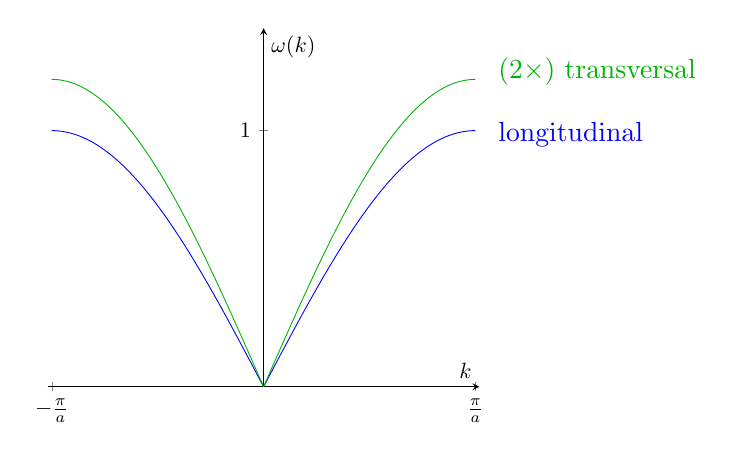
\begin{tikzpicture}[scale=0.8]
        \begin{axis}[
        axis x line=center,
        axis y line=center,
        xlabel= $k$,
        ylabel=$\omega(k)$,
        xmin=-3.2,xmax=3.2,
        ymin=0,ymax=1.4,
        xtick={-3.14,3.14},
        ytick={1},
        xticklabels={$-\frac{\pi}{a}$, $\frac{\pi}{a}$}
        ]
        \addplot[color=blue, samples=100, domain=0:3.141]{sin(deg(x/2))};
        \addplot[color=blue, samples=100, domain=-3.141:0]{-sin(deg(x/2))};
        \addplot[color=green!70!black, samples=100, domain=0:3.141]{1.2*sin(deg(x/2))};
        \addplot[color=green!70!black, samples=100, domain=-3.141:0]{-1.2*sin(deg(x/2))};
        \end{axis}
        \draw[blue] (7,4) node[anchor=west]{longitudinal};
        \draw[green!70!black] (7,5) node[anchor=west]{(2$\times$) transversal };
    \end{tikzpicture}
\end{center}

\subparagraph{1D 2 Atome per Einheitszelle:}
\begin{center}
    \begin{tikzpicture}[scale=0.8]
        \begin{axis}[
        axis x line=center,
        axis y line=center,
        xlabel= $k$,
        ylabel=$\omega(k)$,
        xmin=-3.2,xmax=3.2,
        ymin=0,ymax=2,
        xtick={-3.14,3.14},
        ytick={1},
        xticklabels={$-\frac{\pi}{a}$, $\frac{\pi}{a}$}
        ]
        \addplot[color=blue, samples=100, domain=0:3.141]{sin(deg(x/2))};
        \addplot[color=blue, samples=100, domain=-3.141:0]{-sin(deg(x/2))};
        \addplot[color=green!70!black, samples=100, domain=-3.141:3.141]{0.2*cos(deg(x))+1.5};
        \end{axis}
        \draw[blue] (7,2.9) node[anchor=west]{akustischer Zweig};
        \draw[green!70!black] (7,3.8) node[anchor=west]{optischer Zweig};
    \end{tikzpicture}
\end{center}

\subparagraph{3D p Atome per Einheitszelle:}
\begin{itemize}
    \item $3$ akust. Zweige mit $3N$ akust. Moden
    \item $3(p-1)$ opt. Zweige mit $3N(p-1)$ opt. Moden
\end{itemize}

\paragraph{Statistische Physik}

Innere Energie
\begin{align}
    U=U_0+ \sum_k \expval{n_k} \varepsilon_k = U_0 + \sum_k \frac{\varepsilon_k}{e^{\beta \varepsilon_k}-1} \qquad k=(\Vec{k},\underbrace{s}_{\text{Zweige}})
\end{align}
Wärmekapazität
\begin{align}
    c_V=\left( \pdv{U}{T}\right)_V = \sum \frac{\varepsilon_k (-1) e^{\beta\varepsilon_k}\varepsilon_k \frac{-1}{k_BT^2}}{(e^{\beta \varepsilon_k}-1)^2} = k_B \sum_k \frac{(\beta\varepsilon_k)^2e^{\beta \varepsilon_k}}{(e^{\beta \varepsilon_k}-1)^2}
\end{align}
\begin{enumerate}
    \item hohe Temperaturen $k_B T>>\max_k \varepsilon_k$
        \begin{align}
            &\Rightarrow \beta\varepsilon_k << 1 \Rightarrow e^{\beta\varepsilon_k}=1+\beta\varepsilon + ...\\
            &\Rightarrow c_V = k_B\sum \frac{(\beta\varepsilon_k)^2}{(\beta\varepsilon_k)^2} = k_B \sum_k 1 = 3Nk_B \qq{Dulong-Petit}
        \end{align}
    \item tiefe Temperaturen $k_B T<<\max_k \varepsilon_k$\\
        Nur wenige Beiträge mit $\varepsilon_k \leq k_BT$ wichtig\\
        $\Rightarrow$ nur wenige akustische Zweige $(s=1,2,3)$ mit $\omega(k)=c_S(\Vec{k})\abs{\Vec{k}}$
        \begin{align}
            \sum_k &\rightarrow \underbrace{3}_{\text{Zahl der Zweige}}\underbrace{\frac{1}{\left(\frac{2\pi}{L}\right)^2}}_{\text{Volumen Zelle in k-Raum}}\int_0^{k_{\max}}dk \ 4\pi k^2\\
            c_V &= k_B \frac{12\pi V}{8 \pi^3} \int_0^{k_{\max}} dk \ k^2 \frac{(\beta \hbar ck)^2 e^{\beta \hbar ck}}{(e^{\beta \hbar ck}-1)^2}\\
            &\overset{x=\beta \hbar ck}{=} \frac{3Vk_B}{2\pi^2} \left(\frac{k_BT}{\hbar c}\right)^3 \underbrace{\int_0^{\beta\hbar ck_{\max}\to \infty}dx \frac{x^4 e^x}{(e^x-1)^2}}\\
            &\qquad \stackrel{p.I.}{=} ... \underbrace{\left[x^4 \frac{-1}{e^x-1}\right]_0^\infty}_{=0} + \underbrace{\int_0^\infty dx \ \frac{4 x^3}{e^x-1}}_{=4 \Gamma(4)\zeta(4) = \frac{\pi^4}{15}}\\
            c_V &=\frac{2\pi^2Vk_B}{5} \left(\frac{k_BT}{\hbar c}\right)^3 \sim T^3
        \end{align}
        \begin{center}
        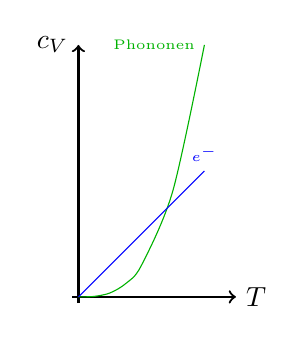
\begin{tikzpicture}[scale=0.8]
            \draw[thick,->] (0,-0.1) -- (0,4) node[anchor=east]{$c_V$};
            \draw[thick,->] (-0.1,0) -- (2.5,0) node[anchor=west]{$T$};
            \draw[green!70!black] plot [smooth] coordinates{(0,0) (0.25,0.0078125) (0.5,0.0625) (0.75,0.2109375) (1,0.5) (1.5,1.6875) (2,4)} node[anchor=east]{\tiny Phononen};
            \draw[blue] (0,0) -- (2,2) node[anchor=south]{\tiny$e^-$};
        \end{tikzpicture}
        \end{center}
        \item allgemein: Debye-Modell
        \begin{itemize}
            \item akustische Zweige mit $\omega=c_D \abs{\Vec{k}}$
            \item Bestimmung von $k_{max} = k_D$
        \end{itemize}
\end{enumerate}
\begin{align}
    \underbrace{\sum_k 1}_{3D} &= 3 \left(\frac{L}{2\pi}\right)^3 \underbrace{4\pi \int_0^{k_{\text{max}}=k_D} dk \, k^2}_{=\frac{4\pi}{3}k_D^3} \\
    &\Rightarrow k_D = \left(6\pi^2\frac{N}{V}\right)^{1/3}\\
    &\Rightarrow c_V = \frac{3 V k_B}{2\pi} \left(\frac{k_B T}{\hbar c}\right)^3 \int_0^{\beta\hbar ck_D}dx \frac{x^4 e^x}{(e^x-1)^2}
\end{align}
\begin{align}
    &\qq{Debye-Frequenz:} \omega_D = c k_D = c k_{max}\\
    &\qq{Debye-Temperatur:} k_B \theta_D = \hbar \omega_D = \hbar c k_D\\
    &\Rightarrow \scalebox{1.1}{\fcolorbox{green!70!black}{white}{$c_V = 9Nk_B \left( \frac{T}{\theta_D}\right)^3 \Big\int_0^{\frac{\theta_D}{T}} dx \frac{x^4 e^x}{(e^x-1)^2}$}}
\end{align}


\begin{center}
        \begin{tikzpicture}[scale=0.8]
            \draw[thick,->] (0,-0.1) -- (0,4) node[anchor=east]{$c_V$};
            \draw[thick,->] (-0.1,0) -- (5,0) node[anchor=west]{$T$};
            \draw[thick] (0.1,3) -- (-0.1,3) node[anchor=east]{$3k_BT$};
            \draw[thick] (1.6,0.1) -- (1.6,-0.1) node[anchor=north]{$\theta_D$};
            \draw[green!70!black] plot [smooth] coordinates{(0,0) (0.25,0.0078125) (0.5,0.0625) (0.75,0.2109375) (1,0.5) (1.5,1.6875) (2,2.4) (2.5,2.8) (3,2.95) (3.5,3) (4,3)};
            \draw (0.4,0.3) node{\tiny$\sim T^3$};
            \draw (3.5,2.8) node{\tiny$\sim T^0$};
        \end{tikzpicture}
\end{center}

\subsection{Wechselwirkende Teilchen} \marginpar{VL 25}
bisher: ideale Gase, d.h. keine WW\\
realistische Systeme: WW oft klein

\subsubsection{Virialentwicklung}
Sei WW kurzreichweitig (z.B. Moleküle eines Gases).
\begin{itemize}
    \item[$\Rightarrow$] bei geringer Dichte $n=\frac{N}{V}$ kleine Störung
    \item[$\rightarrow$] Entwicklung nach kleinen $n$
    \begin{equation}
        \underbrace{\frac{p}{kT} = n}_{\text{ideales Gas}} + \sum_{l=2}^{\infty} \underbrace{B_l(T) \quad n^l}_{\text{Korrektur der Ordnung } l}
    \end{equation}
\end{itemize}

\paragraph{Bemerkung:}
\begin{itemize}
    \item $B_l$ ist $l$-ter Virialkoeffizient
    \item Name wegen Virialsatz: $\expval{E_{kin}} = - \frac{1}{2} \sum_i \expval{\Vec{F}_i\cdot \Vec{r}_i}$
    \item $B_l = B_l(T)$
    \item experimentell werden $B_2(T)$ und $B_3(T)$ bestimmt
\end{itemize}

\paragraph{Frage:} Wie hängen $\underbrace{B_2(T)}_{\text{makroskopisch}}$ mit $\underbrace{\text{WW-Potential } W(\Vec{r})}_{\text{mikroskopisch}}$ zwischen Molekülen zusammen?

\paragraph{Ergebnis:}
\begin{equation}
    \fcolorbox{red}{white}{$B_2(T) = \frac{1}{2} \int_V \, d^3r \ \left(1-e^{-\beta W(\Vec{r})}\right)$}
\end{equation}
\color{black!40} V muss nur WW-Bereich einschließen, da der Integrand sonst annähernd bzw exakt null ist. Daher gibt es keine V Abhängigkeit. \color{black}
\paragraph{Herleitung}
Großkanonische Zustandssumme:
\begin{align}
    Z_G = \Tr\left(e^{-\beta(\hat{H}-\mu \hat{N})}\right) = \sum_{N=0}^{\infty}\underbrace{Z(T,V,N)}_{=: Z_n \text{ kanon.}} e^{\beta\mu N} = \underbrace{Z_0}_{e^{-\beta E_{\text{\tiny Vakuum}}}=1 }+ \sum_{l=1}^{\infty} \, Z_l \, z^l \\
    \qq{mit} z := e^{\beta \mu} \qq{Fugazität} z \ll 1    
\end{align}
Großkanonisches Potential:
\begin{align}
    \Phi &= -pV = -kT \ \ln(Z_G) \\
    &\Rightarrow \frac{pV}{kT} = \ln(Z_G) = \ln\left(1 + \sum_{l=1}^{\infty}\, Z_l \, z^l\right) =: \sum_{l=1}^{\infty}\, a_l \, Z^l \label{4_eq:1_virial} \\
    N &= -\pdv{\Phi}{\mu} = V \pdv{p}{\mu} \stackrel{(\ref{4_eq:1_virial})}{=} V \pdv{p}{z} \underbrace{\pdv{z}{\mu}}_{\beta z} = V \frac{kT}{V} \sum_{l=1}^{\infty} \, a_l \, l \, z^{l-1} \beta z = \sum_{l=1}^{\infty} \, l\,a_l \, z^l \label{4_eq:2_virial}
\end{align}

\subparagraph{1} Bestimme $a_l(Z_1,Z_2,..)$ aus \cref{4_eq:1_virial}:
\begin{align}
    \ln(1+x) &= x - \frac{x^2}{2} + \frac{x^3}{3} -... \qq{mit} x = \sum_{l=1}^{\infty} \, Z_l \, z^l\\
    &\stackrel{\text{bis 2. Ord.}}{=} (Z_1z+Z_2 z^2+..) - \frac{1}{2} (Z_1 z+...)^2 +...\\
    &= \underbrace{Z_1}_{=a_1} + \underbrace{(Z_2 - \frac{1}{2}Z_1^2)}_{= a_2} z^2 + ...
\end{align}

\subparagraph{2} Invertiere \cref{4_eq:2_virial} zu $\sum_{m=1}^{\infty} \, b_m N^m$:
\begin{align}
    (\ref{4_eq:2_virial}): \ N &= 1\cdot a_1 \cdot (b_1N^1+b_2N^2+...)^1 + 2\cdot a_2 \cdot (b_1 N +...)^2 + ...\\
    &= \underbrace{a_1b_1}_{=1}N + \underbrace{(a_2b_2+2a_2b_1^2)}_{=0}N^2+...\\
    &\Rightarrow b_1 = \frac{1}{a_1} \quad b_2 = -\frac{2 a_2b_1^2}{a_1} = -\frac{2a_2}{a_1^3}
\end{align}

\subparagraph{3} Eliminiere damit $z$ in \cref{4_eq:1_virial}:
\begin{align}
    \frac{pV}{kT} &= \sum_{l=1}^{\infty} a_l z^l = a_1(b_1N+b_2N^2+...)+a_2(b_1N+...)^2+...\\
    &= \underbrace{a_1b_1}_{=1} N + \underbrace{(a_1b_2+a_2b_1^2)} N^2 + ...\\
    & - \frac{2a_2}{a_1^2} + \frac{a_2}{a_1^2} = -\frac{a_2}{a_1^2} = - \frac{Z_2 - \frac{1}{2}Z_1^2}{Z_1^2} = \frac{1}{2} - \frac{Z_2}{Z_1^2} \\
    \frac{p}{kT} &= n + \underbrace{V\left(\frac{1}{2}-\frac{Z_2}{Z_1^2}\right)}_{=B_2(T)} n^2+...
\end{align}

\subparagraph{4} Bestimme kanonische Zustandssumme $Z_1,Z_2,...$:
\begin{align}
    &\rightarrow \qq{kline Dichten} n = \frac{N}{V} \qq{im Sinne} \left(\frac{V}{N}\right)^{1/3} \gg \lambda = \frac{h}{\sqrt{2\pi mkT}} \qq{kl. Grenzfall}\\
\end{align}
1 Teilchen:
\begin{align}
    Z_1 &= \frac{1}{h^3} \underbrace{\int d^3q}_{=V} \, \underbrace{\int d^3p \ e^{-\beta \frac{p^2}{2m}} }_{(\sqrt{2\pi mkT})^3} = \frac{V}{\lambda^3} \\
    (\Rightarrow z=b_1N+...&=\frac{1}{a_1}N+...=\frac{1}{Z_1}N+...= \lambda^3 \cdot \frac{N}{V} + ... \ll 1 \Rightarrow z \ll 1 )\\
    &\rightarrow \qq{rechtfertigt Entwicklung in (\ref{4_eq:1_virial}) und (\ref{4_eq:2_virial})}
\end{align}
2 Teilchen:
\begin{align}
    Z_2 &= \frac{1}{2!} \frac{1}{h^6} \int_V d^3q_1 \, \int_V d^3q_2 \, \int d^3p_1 \, \int d^3p_2 e^{-\beta \left(\frac{p_1^2}{2m}+\frac{p_2^2}{2m}+W(\Vec{q}_1 - \Vec{q}_2)\right)} \\
    &W(\Vec{q}_1 - \Vec{q}_2) \qq{Zweiteilchen WW}\\
    &= \frac{1}{2} \frac{(\sqrt{2\pi mkT})^6}{h^6} \underbrace{\int d^3R}_{V} \, \int d^3r \, e^{-\beta W(\Vec{r})} \qq{mit} \Vec{r} = \Vec{q}_1 - \Vec{q}_2, \ \Vec{R} = \frac{\Vec{q}_1 + \Vec{q}_2}{2} \\
    &= \frac{V}{2\lambda^2} \int d^3r e^{-\beta W(\Vec{r})}\\
    &\Longrightarrow B_2(T) = V\left(\frac{1}{2}-\frac{Z_2}{Z_1^2}\right) = \frac{1}{2} \int_V \left(1-e^{-\beta W(\Vec{r})}\right) \quad \checkmark\\
    &\stackrel{W(\Vec{r})=W(r)}{=} 2\pi \int_0^{\infty} dr \, r^2\left(1-e^{-\beta W(r)}\right)
\end{align}

\paragraph{Bemerkung}
\begin{itemize}
    \item Zusammenhang zwischen makroskopischer Messgröße und mikroskopischer Eigenschaft
    \item ideales Gas $\Rightarrow$ keine WW $\Rightarrow \ W(\Vec{r})=0 \ \Rightarrow \ B_2(T)=0 \ \Rightarrow \ \frac{p}{kT}=n \ \checkmark$
    \item typisches WW-Potential:
    \begin{center}
        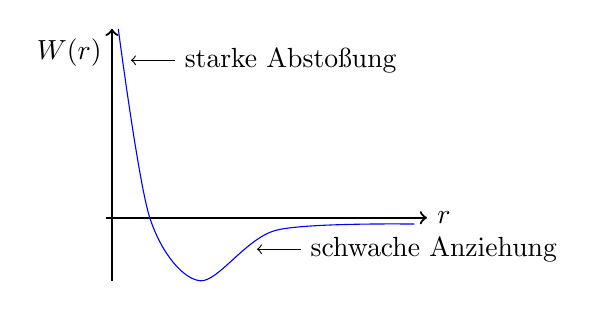
\begin{tikzpicture}[scale=0.8]
            \draw[thick,->] (0,-1) -- (0,3) node[anchor=north east]{$W(r)$};
            \draw[thick,->] (-0.1,0) -- (5,0) node[anchor=west]{$r$};
            \draw[blue] plot [smooth] coordinates{(0.1,3) (0.6,0) (1.4,-1) (2.6,-0.2) (4.8,-0.1)};
            \draw[<-] (2.3,-0.5) -- (3,-0.5) node[anchor=west]{schwache Anziehung};
            \draw[<-] (0.3,2.5) -- (1,2.5) node[anchor=west]{starke Abstoßung};
        \end{tikzpicture}
    \end{center}
    \item empirischer Ansatz: \emph{Lennard-Jones-Potential}
    \begin{equation}
        W(r) = 4\varepsilon \left[\left(\frac{r_0}{r}\right)^{12} - \left( \frac{r_0}{r}\right)^6\right] 
    \end{equation}
    \begin{itemize}
        \item[] Parameter: $\varepsilon,r_0$ können experimentell aus $B_2(T)$ bestimmt werden
        \item identisch mit van-der-Waals-Zustandsgleichung bis 2. Ordnung
        \item van-der-Waals kann mehr, z.B. Phasenübergang flüssig $\leftrightarrow$ gasförmig
        \item auch für Quantengase möglich, allerdings entsprechen die idealen Quantengase den virial genäherten Gasen mit Potential (Fermionen: abstoßend, Bosonen: anziehend)
    \end{itemize}
\end{itemize}

\subsubsection{Ferromagnetismus, Ising-Modell} \marginpar{VL 26}

\begin{tabular}{ccc}
     \textbf{Ferromagneten (Fe,Co,Ni,...)} & $\Leftrightarrow$ & \textbf{Paramagneten / Diamagneten }  \\
     & & \color{black!40} $\chi > 0$ / $\chi<0$\\
     Magnetisierung ohne Magnetfeld & & Magnetisierung $\propto$ Magnetfeld\\
     &&\\
     WW zwischen den Spins & & keine WW\\
     &&\\
     \textcircled{$\uparrow$} & &$\Vec{M} = \chi\Vec{B}$
\end{tabular}

\textbf{Ziel:} Erklärung Ferromagnetismus durch mikroskopische Theorie

\begin{prop}{Hamilton-Operator}
    \begin{equation}
        \Hat{H} = - g\, \mu_B \Vec{B} \sum_{i=1}^N \Vec{S}_i - \sum_{\substack{i,j\\i<j}} J_{ij} \, \Vec{S}_i \cdot \Vec{S}_j
    \end{equation}
    \begin{itemize}
        \item[$g$] - Landé-Faktor (=2)
        \item[$\mu_B$] - Bohr'sches Magneton
    \end{itemize}
\end{prop}

\paragraph{Ordnungsparameter} Magnetisierung:
\begin{equation}
    \Vec{M} = \frac{1}{V} g \mu_B \sum_{i=1}^N \Vec{S}_i
\end{equation}

\paragraph{Heisenberg-Modell} (nur WW nächster Nachbarn)
\begin{align}
    H_{\text{Heisenberg}} = -g\mu_B \Vec{B} \sum_{i=1}^N \Vec{S}_i - J \sum_{\substack{\expval{i,j}\\\text{nächste}\\\text{Nachbarn}}} \Vec{S}_i \cdot \Vec{S}_j
\end{align}

\paragraph{Molekularfeldnäherung} (Weiss 1907) \say{mean field theory}:
\begin{itemize}
    \item Betrachtung Betrag von Spin i:
    \begin{equation}
        H_i = - \Vec{S}_i \underbrace{\left[g\mu_B\Vec{B}+J \sum_{\expval{i,j}} \Vec{S}_j\right]}_{=: g\mu_B \Vec{B}_{eff}^{(i)}}
    \end{equation}
    \item Molekularfeldnäherung:
    \begin{align}
        \Vec{B}_{eff} &= \expval{\Vec{B}_{eff}^{(i)}}_i \\
        &= \Vec{B} + \frac{J}{g\mu_B} \underbrace{\expval{\sum_{\expval{i,j}} \Vec{S}_j}_i}_{\propto \Vec{M}} = \Vec{B} + \lambda \Vec{M}
    \end{align}
    \item[$\Rightarrow$] $H_{MFN}$ mit Selbstkonsistenz von $\Vec{M}$
\end{itemize}
\subparagraph{Freie Energie:}
\begin{align}
    F_{MFN} &= NkT \left\{ \frac{1}{2} \frac{T_c}{T} \left(\frac{M}{M_\infty}\right)^2 - \ln \left[ 2 \cosh\left( \frac{g\mu_BB}{2kT}+\frac{T_c}{T} \frac{M}{M_\infty}\right)\right]\right\}\\
    T_c &= \frac{Jp}{4k} \qq{p - Zahl der Nachbarn}\\
    M_\infty &= \frac{Ng\mu_B}{2V} \qq{Sättigungsmagnetisierung}\\
    B=0, \ \frac{M}{M_\infty} \ll 1: \quad F &= NkT \left[ -\ln(2) + \frac{1}{2} \frac{T_c}{T} \left(1-\frac{T_c}{T}\right) \left(\frac{M}{M_\infty}\right)^2 + \frac{1}{12} \left(\frac{T_c}{T}\right)^4 \left(\frac{M}{M_\infty}\right)^4+...\right]
\end{align}

\begin{center}
    \begin{tikzpicture}[scale=0.8]
    \begin{axis}[
    axis lines = left,
    xlabel = $M$,
    ylabel = $F$,
    xmin = -2.5, xmax = 2.5,
    ymin=0, ymax=2.5,
    xtick={0},
    ytick=\empty,
    ]
    \addplot[blue, samples=100, domain=-1.2:1.2]{x^2+0.8};
    \end{axis}
    \draw[blue] (3.5,3.5)node{$T>T_c$};
    \end{tikzpicture}
    \hspace{1.5cm}
    \begin{tikzpicture}[scale=0.8]
    \begin{axis}[
    axis lines = left,
    xlabel = $M$,
    ylabel = $F$,
    xmin = -2.5, xmax = 2.5,
    ymin=0, ymax=3,
    xtick={0},
    ytick=\empty,
    ]
    \addplot[blue, samples=100, domain=-1.6:1.6]{-2*x^2+x^4+1.5};
    \end{axis}
     \draw[blue] (3.5,3.5)node{$T<T_c$};
    \end{tikzpicture}
\end{center}
\begin{center}
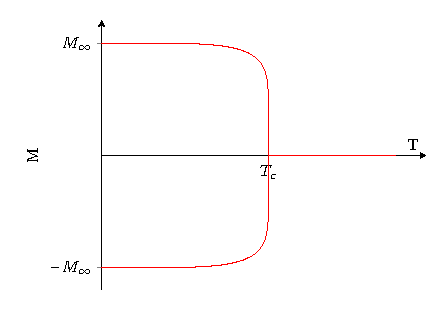
\includegraphics{Tikz Standalone/Tikz_magnetisierung.pdf}
\end{center}

\begin{itemize}
    \item[$\rightarrow$] Phasenübergang:
    \begin{itemize}
        \item $M$: Ordnungsparameter (genauer: $\expval{M}$)
        \item $T>T_c$: symmetrische oder ungeordnete Phase ($H$ ist rotationssymmetrisch, $S$ auch)
        \item $T<T_c$: spontane Symmetriebrechung,geringe Symmetrie, alle Spins ausgerichtet)
    \end{itemize}
    \item[$\rightarrow$] Physenübergang 2. Ordnung:
    \begin{itemize}
        \item Ordnungsparameter stetig (1. Ableitung unstetig)
        \item Phasen nicht gleichzeitig existent
        \item keine Umwandlungswärme notwendig
    \end{itemize}
    \item allgemein: \emph{Landau-Theorie der Phasenübergänge} (\say{Universalitätsklassen})
\end{itemize}

\paragraph{Ising-Modell}
\begin{center}
\emph{Motivation}: vollständig lösbares Modell des Ferromagnetismus mit Phasenübergang (\say{Es könnte ja sein, dass der Phasenübergang aus MFN resultiert.})
\end{center}
Heisenbergmodell ohne $x$- und $y$-Komponente des Spins:
\begin{equation}
    H = -g\mu_B B_z \sum_i S_i^z - J \sum_{\expval{i,j}} S_i^z S_j^z \qquad J > 0
\end{equation}
\begin{itemize}
    \item in diesem Modell alle Mikrozustände / Eigenzustände bekannt
    \item $S_i^z$ vertauschen mit Hamilton-Operator
    \begin{itemize}
        \item[$\Rightarrow$] Eigenzustände von $H$ sind beliebige Konfigurationen der Spins
        \begin{equation}
            \qq{mit} \ket{+} \ (\sigma = +1) \qq{oder} \ket{-} \ (\sigma = -1)
        \end{equation}
        \item[$\Rightarrow$] Energie einer Spinkonfiguration:
        \begin{equation}
            E(\{\sigma_i\}) = - \Tilde{B} \sum_i \sigma_i - \Tilde{J} \sum_{\expval{i,j}} \sigma_i\sigma_j
        \end{equation}
    \end{itemize}
    \item[1D]: exakte Lösung, kein Phasenübergang, kein Ferromagnetismus
    \item[2D]: Ising-Modell für $\Tilde{B}=0$
    \item[] Onsager 1944: (Zustandsumme + freie Energie)
    \begin{itemize}
        \item[$\Rightarrow$] Phasenübergang:
        \begin{equation}
            \sinh\left(\frac{2\Tilde{J}}{kT_c}\right) = 1 \qquad \Rightarrow \quad T_c = 2,269...\cdot \frac{\Tilde{J}}{k}
        \end{equation}
    \end{itemize}
    \item[] Young 1952:
    \begin{equation}
        M(T,B=0) \propto \expval{\sigma_i} = \begin{cases}
            \qquad \qq{0}\qquad \qq{      }, T>T_c\\
            \pm \left(1-\frac{1}{\sinh^4\left(\frac{2\Tilde{J}}{kT}\right)}\right)^{1/8} \ , T<T_c
        \end{cases}
    \end{equation}
\end{itemize}

\begin{center}
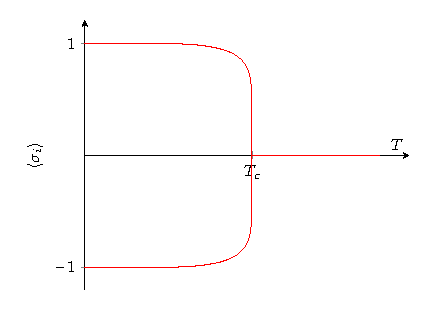
\includegraphics{Tikz Standalone/Tikz_spin.pdf}
\end{center}

Numerik:
\begin{itemize}
    \item dimensionslose Temperatur:
    \begin{align}
        \tau :&= \frac{T}{\frac{\Tilde{J}}{k}}\\
        \tau_c :&= \frac{T_c}{\frac{\Tilde{J}}{k}} = 2,269...
    \end{align}
\end{itemize}